%------------------------------------------------------------------------------%
\section{The Axioms of ZF}
    The first thing to do is define what \textit{sets} are. These are the
    most fundamental and basic structures in mathematics.
    \begin{fdefinition}{Sets}{Sets}
        A set is a collection of objects (or elements),
        none of which is the set itself.
    \end{fdefinition}
    If we wish to stand on a truly solid foundation, it seems we're off to a
    bad start. In the definition of sets we used the words \textrm{collection}
    and \textrm{objects}, neither of which we have defined. If we attempt to
    define these terms we would almost certainly run into the same problem,
    and thus we can't proceed until we define the entire English language.
    Even if we were to do such a task, we'd inevitably end up with circular
    definitions. To begin stating definitions and theorems we need the
    existence of a \textit{thing}. Sets act as our thing. We know they exist,
    but we don't know how to define them all to well. Nevertheless, we can
    describe how they behave and what they can do, as well as how to obtain
    new sets from pre-existing ones. This is what the axioms of
    Zermelo-Fraenkel set theory aim to do.
    \begin{fnotation}{Element Notation}{Element_Notation}
        If $A$ is a set and if $x$ is an element of $A$, then we denote this
        by writing $x\in{A}$. If $x$ is not an element of $A$, we write
        $x\notin{A}$.
    \end{fnotation}
    As of yet we do not know that any sets exist. Pedagogically it seems poor
    to wait to show examples, so we'll speak loosely for the moment to allow
    one to familiarize themselves with the notation.
    \begin{lexample}{Using Element Notation}{Using_Element_Notation}
        Given a set $A$ that contains only a few objects, we can represent
        $A$ by listing out the elements, separated by commas, and enclosing
        them in braces. Suppose $A$ is the set that contains three distinct
        objects, labelled $a$, $b$, and $c$. We then write:
        \begin{equation}
            A=\{\,a,\,b,\,c\,\}
        \end{equation}
        If we are told that there is a fourth object $d$ that is different
        from $a$, $b$, and $c$, then we can use the notation defined in
        Not.~\ref{not:Element_Notation} to write the following:
        \par\hfill\par
        \begin{subequations}
            \begin{minipage}[b]{0.49\textwidth}
                \begin{equation}
                    a\in{A}
                \end{equation}
            \end{minipage}
            \hfill
            \begin{minipage}[b]{0.49\textwidth}
                \begin{equation}
                    d\notin{A}
                \end{equation}
            \end{minipage}
        \end{subequations}
        \par\vspace{2.5ex}
        The notation $a\in{A}$ should be read as \textit{a is an element of A},
        or \textit{a is contain in A}, or simply \textit{a is in A}. Similarly,
        the notation $d\notin{A}$ should be read as
        \textit{d is not an element of A}, or \textit{d is not contained in A}.
    \end{lexample}
    The example shown in Ex.\ref{ex:Using_Element_Notation} is
    \textit{finite}. Moreover it contains only three elements. For larger sets
    we rely on other methods to write them down. One such means is to indicate
    a pattern and use an ellipses to show that it goes on. Such a description
    is vague and lacks rigor, but can be helpful when the pattern is obvious.
    \begin{lexample}{More Examples of Element Notation}
                    {More_Examples_of_Element_Notation}
        The set of all \textit{natural} numbers, or non-negative integers,
        will soon be the center of attention as we use the laws of set theory
        to prove its existence and unveil many properties. We use the symbol
        $\mathbb{N}$ to denote this set. We can write:
        \begin{equation}
            \label{eqn:Natural_Numbers_Ellipses}%
            \mathbb{N}=\{\,0,\,1,\,2,\,3,\,4,\,5,\,\dots\,\}
        \end{equation}
        Using our developed notation, we can write:
        \par\hfill\par
        \begin{subequations}
            \begin{minipage}[b]{0.49\textwidth}
                \begin{equation}
                    23\in\mathbb{N}
                \end{equation}
            \end{minipage}
            \hfill
            \begin{minipage}[b]{0.49\textwidth}
                \begin{equation}
                    \minus{4}\notin\mathbb{N}
                \end{equation}
            \end{minipage}
        \end{subequations}
        \par\vspace{2.5ex}
        If we let $\mathbb{Z}_{n}$ denote all non-negative integers
        between $0$ and $n-1$, we can write:
        \begin{equation}
            \label{eqn:Z_n_Ellipses}%
            \mathbb{Z}_{n}=\{0,\,1,\,2,\,\dots,\,n-1\,\}
        \end{equation}
        Using this we find that $17\in\mathbb{Z}_{18}$ but
        $19\notin\mathbb{Z}_{18}$. Finally, we present the integers.
        \begin{equation}
            \label{eqn:Integers_Ellipses}%
            \mathbb{Z}=\{\,\dots,\,\minus{3},\,\minus{2},\,\minus{1},
                            \,0,\,1,\,2,\,3,\dots\,\}
        \end{equation}
    \end{lexample}
    In our definition of a set (Def.~\ref{def:Sets}), we explicitly
    required that sets cannot contain themselves. That is, if
    $A$ is a set, then $A\notin{A}$. This requirement was introduced to
    avoid paradoxes discovered by Bertrand Russell in 1901. Allow us to
    neglect this requirement, for a moment, to reveal why it is essential.
    Let's call a system of mathematics inconsistent if one can prove
    a contradiction within the theory. In Naive Set Theory we allow the
    \textit{axiom of unrestricted comprehension}. This allows us to
    constructs sets as any defineable collection. That is, if we have a
    proposition $P$, then we can define a set $A$ as the set of all objects
    that satisfy $P$. We can write:
    \begin{equation}
        A=\{\,x\;|\;P(x)\,\}
    \end{equation}
    Problems with such a loose definiton arise instantly. Let $P$ be the
    proposition \textit{true if x is a set, false otherwise}. Then
    $A=\{\,x\;|\;P(x)\,\}$ can be read in plain English as the
    \textit{set of all sets}. A natural question would be whether or not
    $A$ then contains itself. That is, is $A\in{A}$? Russell's paradox
    arises by defining proper sets to be sets $B$ such that $B\notin{B}$,
    and improper sets to be sets $B$ such that $B\in{B}$. Using the
    \textit{Law of the Excluded Middle} (which we will prove later), one
    has that every set is either proper or improper.
    \begin{ftheorem}{Russell's Paradox}{Russell_Paradox}
        Naive Set Theory is inconsistent.
    \end{ftheorem}
    \begin{bproof}
        For let $P$ be the proposition
        \textit{true if} $x\notin{x}$, \textit{false otherwise}.
        Let $A$ be the set defined by this proposition:
        \begin{equation}
            A=\{\,x\;|\;P(x)\,\}
        \end{equation}
        That is, $A$ is the set of all sets that do not contain themselves.
        Suppose $A\in{A}$. If $A\in{A}$ then $P(A)$ is true. That is, $A$ is a
        proper set. But proper sets do not contain themselves and $A\in{A}$, a
        contradiction. Thus $A\notin{A}$. But if $A\notin{A}$ than $P(A)$ is
        false. But if $P(A)$ is false, than $A$ is a improper set. But then
        $A\in{A}$, a contradiction as $A\notin{A}$. Thus $A\in{A}$ if and only
        if $A\notin{A}$, a contradiction. Therefore, Naive Set Theory is
        inconsistent.
    \end{bproof}
    Our development of Zermelo-Fraenkel Set Theory is to avoid this
    paradox and attempt to develop a consistent system of mathematics.
    The first collection of axioms was proposed in 1908 by Ernst
    Zermelo. Subtle problems were pointed out by Abraham Fraenkel
    in 1920, and in 1921 the system of Zermelo-Fraenkel set theory came
    to be. Combining this with the axiom of choice creates the system
    commonly abbreviated as ZFC.
    \par\hfill\par
    The requirement that a set does not contain itself is sufficient to
    avoid Russell's paradox. This is usually stated as the
    \textit{axiom of regularity}. To avoid circular reasoning, we will
    prove the equivalence of this axiom with our definition once the law
    of the excluded middle has been proved. We will first develop the
    other axioms and construct some of the basic objects of set theory.
    \subsection{Subsets and Equality}
        To delve more into set theory it would be convenient to know that
        at least \textit{one} set exists. The axiom of the empty set gives
        us such an existance.
        \begin{faxiom}{Axiom of the Empty Set}{Axiom_of_the_Empty_Set}
            There exists a set $\emptyset$ (the empty set) such
            that for all $x$ it is true that $x\notin\emptyset$.
        \end{faxiom}
        The empty set is the set that contains no elements. As such, some
        choose to write $\emptyset=\{\}$. Note that the empty set is
        different from the set $\{\emptyset\}$. The empty set contains no
        elements whereas $\{\emptyset\}$ contains one elements (it
        contains the empty set). Indeed, the equality of $\emptyset$ and
        $\{\emptyset\}$ would violate our requirement that sets do not
        contain themselves.
        \par\hfill\par
        A set is entirely determined by its elements, and as such
        repetition and order cannot be accounted for. That is, the sets
        $\{\,a,\,b\,\}$ and $\{\,a,\,a,\,b\,\}$ must be considered the same
        since they contain precisely the same elements. This will be made clear
        once equality has been defined. In a similar manner, the sets
        $\{\,a,\,b\,\}$ and $\{\,b,\,a\,\}$ are equivalent. Sets have no notion
        of order. It then becomes a task to invent some new object that does
        have a sense of order. To do this requires the notion of
        \textit{function}, and it is our current aim to develop this topic
        using axiomatic set theory.
        \par\hfill\par
        To rigorously show that the examples in the previous paragraph are
        equal requires a definition of equality. This is phrased in
        Zermelo-Fraenkel set theory as the \textit{axiom of extensionality}.
        \begin{axiom}[Axiom of Extensionality]
            If $A$ and $B$ are sets, and if for all $x$, $x\in{A}$
            if and only if $x\in{Y}$, then $A=B$. That is,
            $A$ and $B$ are equal sets.
        \end{axiom}
        We won't adopt this axiom directly, but rather restate equality
        as a definition using the language of subsets. This will make
        proving various things easier in the proceeding sections. The
        two notions are equivalent.
        Subsets are sets that are defined in terms of another given set
        by simply removing some (or none, or all) of the elements.
        We define this as follows:
        \begin{fdefinition}{Subsets}{Subsets}
            A subset of a set $B$ is a set $A$ such that for all
            $x\in{A}$, it is true that $x\in{B}$. If $A$ is a subset
            of $B$, we write $A\subseteq{B}$. Otherwise, we write
            $A\nsubseteq{B}$.
        \end{fdefinition}
        We can often visualize sets as blobs in the plane. We can use
        such a visual to represent what subsets are as well
        (Fig.~\ref{fig:Subset_Blobs}). Given a blob $B$, a subset of
        $B$ is another blob $A$ that is entirely contained within $B$.
        \begin{figure}[H]
            \centering
            %--------------------------------Dependencies----------------------------------%
%   tikz                                                                       %
%-------------------------------Main Document----------------------------------%
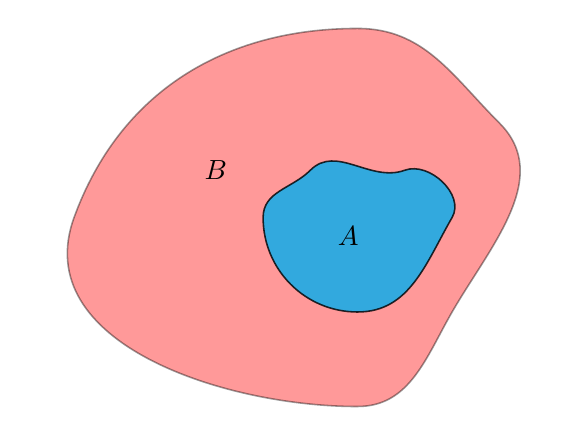
\begin{tikzpicture}[line width=0.2mm, scale=1.2]

    % Coordinates for the bigger blob.
    \coordinate (P1) at ( 0.0, -2.0);
    \coordinate (P2) at ( 1.0, -1.0);
    \coordinate (P3) at ( 1.5,  1.0);
    \coordinate (P4) at ( 0.0,  2.0);
    \coordinate (P5) at (-3.0,  0.0);

    % Coordinates for the inner blob.
    \coordinate (Q1) at ( 0.0, -1.0);
    \coordinate (Q2) at ( 1.0,  0.0);
    \coordinate (Q3) at ( 0.5,  0.5);
    \coordinate (Q4) at (-0.5,  0.5);
    \coordinate (Q5) at (-1.0,  0.0);

    % Coordindates to label things.
    \coordinate (A) at (-0.1, -0.2);
    \coordinate (B) at (-1.5,  0.5);

    % Draw the bigger blob.
    \draw[fill=red, opacity=0.4] (P1) to [out=0,    in=-120] (P2)
                                      to [out=60,   in=-45]  (P3)
                                      to [out=135,  in=0]    (P4)
                                      to [out=-180, in=70]   (P5)
                                      to [out=-110, in=-180] cycle;

    % Draw the inner blob.
    \draw[fill=cyan, opacity=0.8] (Q1) to [out=0,    in=-120]  (Q2)
                                       to [out=60,   in=20]    (Q3)
                                       to [out=-160, in=45]    (Q4)
                                       to [out=-135, in=90]    (Q5)
                                       to [out=-90,  in=180]   cycle;

    % Labels for the two blobs.
    \node at (A) {$A$};
    \node at (B) {$B$};
\end{tikzpicture}

            \caption[Visual for Subsets]
                    {Sets can be Visualized as Blobs in the Plane.}
            \label{fig:Subset_Blobs}
        \end{figure}
        We can use subsets to define equality and to provide examples
        of the \textit{axiom schema of specification}. We will do this,
        but first provide examples of subsets.
        \begin{lexample}{Examples of Subsets}{Examples_of_Subsets}
            Using the notation we developed in
            Ex.~\ref{ex:More_Examples_of_Element_Notation}, we see that
            for all $n\in\mathbb{N}$, we have:
            \begin{equation}
                \mathbb{Z}_{n}\subseteq\mathbb{N}
            \end{equation}
            Define $\mathbb{N}_{e}$ and $\mathbb{N}_{o}$ to be the even
            and odd non-negative integers, respectively:
            \par
            \begin{subequations}
                \begin{minipage}[b]{0.49\textwidth}
                    \begin{equation}
                        \label{eqn:Even_Pos_Ints_Ellipses}%
                        \mathbb{N}_{e}=\{\,0,\,2,\,4,\,6,\,8,\,\dots\,\}
                    \end{equation}
                \end{minipage}
                \hfill
                \begin{minipage}[b]{0.49\textwidth}
                    \begin{equation}
                        \label{eqn:Odd_Pos_Ints_Ellipses}%
                        \mathbb{N}_{o}=\{\,1,\,3,\,5,\,7,\,9,\,\dots\,\}
                    \end{equation}
                \end{minipage}
            \end{subequations}
            \par\vspace{2.5ex}
            From this we see the following two expressions are true:
            \par\hfill\par
            \begin{subequations}
                \begin{minipage}[b]{0.49\textwidth}
                    \begin{equation}
                        \mathbb{N}_{o}\subseteq\mathbb{N}
                    \end{equation}
                \end{minipage}
                \hfill
                \begin{minipage}[b]{0.49\textwidth}
                    \begin{equation}
                        \mathbb{N}_{e}=\mathbb{N}
                    \end{equation}
                \end{minipage}
            \end{subequations}
            \par\vspace{2.5ex}
            Moreover we see that $\mathbb{N}_{o}$ and $\mathbb{N}_{e}$
            have no elements in common. That is, they are
            \textit{disjoint}. We can represent this symbolically by
            writing:
            \par\hfill\par
            \begin{subequations}
                \begin{minipage}[b]{0.49\textwidth}
                    \begin{equation}
                        \mathbb{N}_{o}\nsubseteq\mathbb{N}_{e}
                    \end{equation}
                \end{minipage}
                \hfill
                \begin{minipage}[b]{0.49\textwidth}
                    \begin{equation}
                        \mathbb{N}_{e}\nsubseteq\mathbb{N}_{o}
                    \end{equation}
                \end{minipage}
            \end{subequations}
            \par\vspace{2.5ex}
            We can also think of trivial examples. We see that
            $\mathbb{Z}_{3}\subseteq\mathbb{Z}_{4}$ since every element
            of $\mathbb{Z}_{3}$ is contained in $\mathbb{Z}_{4}$, but
            $\mathbb{Z}_{4}\nsubseteq\mathbb{Z}_{3}$ since
            $3\in\mathbb{Z}_{4}$ but $3\notin\mathbb{Z}_{3}$. It may seem
            like bad notation to write $3\notin\mathbb{Z}_{3}$, but since we
            want $\mathbb{Z}_{n}$ to have $n-\textrm{many}$ elements. Since we
            started counting at zero, $n\notin\mathbb{Z}_{n}$ for all
            $n\in\mathbb{N}$. Such counting schemes are common in computer
            science, but there's disagreement in mathematics as to whether
            $0\in\mathbb{N}$ or not. We will later use the
            \textit{axiom of infinity} to prove the existence of $\mathbb{N}$,
            and in doing so it become very natural to define $\mathbb{N}$ as
            a set that contains $0$.
        \end{lexample}
        The final example shown in Ex.~\ref{ex:Examples_of_Subsets}
        shows how we can define equality of sets. We see that
        $\mathbb{Z}_{3}\subseteq\mathbb{Z}_{4}$, but
        $\mathbb{Z}_{4}\nsubseteq\mathbb{Z}_{3}$. If we have two sets
        $A$ and $B$ such that $A\subseteq{B}$ and $B\subseteq{A}$ then
        it would be impossible to discern between the two.
        \begin{fdefinition}{Equal Sets}{Equal_Sets}
            Equal sets are sets $A$ and $B$, denoted $A=B$, such that
            $A\subseteq{B}$ and $B\subseteq{A}$.
        \end{fdefinition}
        If $A$ and $B$ are not equal, we write $A\ne{B}$.
        Def.~\ref{def:Equal_Sets} is equivalent to the axiom of
        extensionality, but creates a few problems. As discussed
        previously, sets have no notion of order and cannot account
        for repetition.
        \begin{lexample}{Sets Do Not Have Order}{Sets_Do_Not_Have_Order}
            Let $A$, $B$, and $C$ be the sets defined by:
            \par
            \begin{subequations}
                \begin{minipage}[b]{0.32\textwidth}
                    \begin{equation}
                        A=\{\,a,\,b\,\}
                    \end{equation}
                \end{minipage}
                \hfill
                \begin{minipage}[b]{0.32\textwidth}
                    \begin{equation}
                        B=\{\,a,\,a,\,b\,\}
                    \end{equation}
                \end{minipage}
                \hfill
                \begin{minipage}[b]{0.32\textwidth}
                    \begin{equation}
                        C=\{\,b,\,a\,\}
                    \end{equation}
                \end{minipage}
            \end{subequations}
            \par\vspace{2.5ex}
            All three of these sets are equal by both the definition of
            equality (Def.~\ref{def:Equal_Sets}) and the axiom of
            extensionality. It seems clear that $A\subseteq{B}$, but it is
            also true that $B\subseteq{A}$. This is because $B$ contains only
            the elements $a$ and $b$. While $a$ is included twice,
            repetition cannot be accounted for and $B$ is entirely
            determined by $a$ and $b$. But $A$ also contains $a$ and $b$, and
            therefire $B\subseteq{A}$. By the definition of equality
            (Def.~\ref{def:Equal_Sets}), we have that $A=B$. In a similar
            manner, $A=C$.
        \end{lexample}
        From the definition of subsets, for any set $A$ we see that
        $A\subseteq{A}$ (To be proven later). It would be nice to distinguish
        between subsets that aren't the entire set itself. These are called
        proper subsets, and we can define them in terms of equality.
        \begin{fdefinition}{Proper Subsets}{Proper_Subsets}
            A proper subset of a set $B$ is a set $A$ such that
            $A\subseteq{B}$ and $A\ne{B}$. We write $A\subsetneq{B}$
            to denote that $A$ is a proper subset of $B$.
        \end{fdefinition}
        The symbols $\subseteq$ and $\subsetneq$ are analogous to the
        notations of inequalities that one finds in calculus: $\leq$ and $<$.
        In many texts, the two symbols $\subseteq$ and $\subset$ are taken to
        be identical, which may cause confusion. In an attempt to reduce
        confusion, $\subseteq$ will denote any subset, $\subsetneq$ denotes a
        proper subset, and the symbol $\subset$ will be avoided.
        \begin{lexample}{Proper Subsets}{Proper_Subsets}
            Let $A$ and $B$ be sets defined as follows:
            \par
            \begin{subequations}
                \begin{minipage}[b]{0.49\textwidth}
                    \centering
                    \begin{equation}
                        A=\{\,a,\,b,\,c\,\}
                    \end{equation}
                \end{minipage}
                \hfill
                \begin{minipage}[b]{0.49\textwidth}
                    \centering
                    \begin{equation}
                        B=\{\,a,\,b,\,c,\,d\,\}
                    \end{equation}
                \end{minipage}
            \end{subequations}
            \par\vspace{2.5ex}
            Then $A\subseteq{B}$, since every element of $A$ is an
            element of $B$, but $B\nsubseteq{A}$ since $d\in{B}$ and
            $d\notin{A}$. Therefore $A\ne{B}$, and thus $A$ is a proper
            subset of $B$. We can denote this by writing $A\subsetneq{B}$.
        \end{lexample}
        Next, we introduce the \textit{axiom schema of specification},
        develop set-builder notation.
        \begin{faxiom}{Axiom Schema of Specification}
                      {Axiom_Schema_of_Specification}
            If $A$ is a set and if $P$ is a proposition, then there exists
            a set $B$ such that $x\in{B}$ if and only if $x\in{A}$ and
            $P(x)$ is true. We can write this as:
            \begin{equation}
                B=\{\,x\in{A}\,:\,P(x)\,\}
            \end{equation}
        \end{faxiom}
        Ax.~\ref{ax:Axiom_Schema_of_Specification} is different from the
        inconsistent axiom of unrestricted comprehension in that we can only
        speak of elements that are already defined and contained in some other
        set. That is, this new axiom does not allow us to talk about the
        \textit{set of all sets}, and so we have avoided the crux of
        Russell's paradox.
        \par\hfill\par
        This axiom states that the Set-Builder method of constructing
        sets is valid. We have seen that the natural numbers
        $\mathbb{N}$ and the integers $\mathbb{Z}$ (From the German
        \textit{Zahl}) can be loosely described by using ellipses
        (Eqns.~\ref{eqn:Natural_Numbers_Ellipses} and
        \ref{eqn:Integers_Ellipses}, respectively). It would be more
        difficult (but not impossible) to describe the set of rational
        numbers in such a way. Instead, we use set builder notation. We
        can describe the set of rational numbers $\mathbb{Q}$ if it is known
        that there is some larger set $\mathbb{R}$ (the \textit{real} numbers)
        as follows:
        \begin{equation}
            \mathbb{Q}=\Big\{\;\frac{p}{q}\in\mathbb{R}\;|
                               \;p,\,q\in\mathbb{Z}
                               \textrm{ and }q\ne{0}\;\Big\}
        \end{equation}
        That is, the rational numbers are the set of all real numbers which
        can be written as the ratios of integers with non-zero denominator.
        The Axiom Schema of Specification states that this is is a valid
        method of describing sets. It is also known as the axiom of
        separation.
        \begin{lexample}{Set-Builder Notation}{Set_Builder_Evens_and_Odds}
            We can describe the sets $\mathbb{Z}$, $\mathbb{N}$,
            $\mathbb{N}_{e}$, and $\mathbb{N}_{o}$ using set-builder
            notation if we assume these belong to some larger set
            $\mathbb{R}$. We define $\mathbb{Z}$ by:
            \begin{equation}
                \mathbb{Z}=\{\,n\in\mathbb{R}\;|\;
                               n\textrm{ is an integer}\,\}
            \end{equation}
            From here we can define $\mathbb{N}$ by:
            \begin{equation}
                \mathbb{N}=\{\,n\in\mathbb{Z}\;|\;n\geq{0}\,\}
            \end{equation}
            Furthermore, $\mathbb{N}_{e}$ and $\mathbb{N}_{0}$ can be
            described as follows:
            \par
            \begin{subequations}
                \begin{minipage}[b]{0.49\textwidth}
                    \centering
                    \begin{equation}
                        \label{eqn:Even_Pos_Ints_Set_Builder}%
                        \mathbb{N}_{e}=\{\,n\in\mathbb{N}\;|\;
                                           n\textrm{ is even.}\,\}
                    \end{equation}
                \end{minipage}
                \hfill
                \begin{minipage}[b]{0.49\textwidth}
                    \centering
                    \begin{equation}
                        \label{eqn:Odd_Pos_Ints_Set_Builder}%
                        \mathbb{N}_{o}=\{\,n\in\mathbb{N}\;|\;
                                           n\textrm{ is odd.}\,\}
                    \end{equation}
                \end{minipage}
            \end{subequations}
            \par\vspace{2.5ex}
            Such notation is justified by the axiom schema of
            specification. It is important to note that these are not the
            definitions we are adopting since they lack rigor in many respects.
            These examples are simply to build intuition behind the notation
            and the axioms. We will develop $\mathbb{N}$ from a purely
            axiomatic viewpoint shortly, and from there we will construct
            $\mathbb{Z}$, $\mathbb{N}_{e}$, and $\mathbb{N}_{o}$.
        \end{lexample}
    \subsection{Ordered Pairs and Cartesian Products}
        We now wish to solve the issue previously raised that sets do
        not have order. We'll develop a new object, called ordered pairs, that
        can distinguish such things. The definition we'll adopt is due to
        Kuratowski and uses the following form:
        \begin{equation}
            (a,\,b)=\big\{\,a,\,\{\,a,\,b\,\}\,\big\}
        \end{equation}
        We now prove such a set exists within the framework of ZFC.
        \begin{faxiom}{Axiom of Pairing}{Axiom_of_Pairing}
            If $A$ and $B$ are sets, then there exists a set $C$ such that
            $A\in{C}$ and $B\in{C}$.
        \end{faxiom}
        The set hypothesized to exist in this axiom may be very large, we have
        no way of knowing. What we want from this is a set that contains two
        elements $a$ and $b$, and only those elements. Such a set can be proven
        to exists if we combine pairing with the specification.
        \begin{theorem}
            \label{thm:Existence_of_Set_Built_from_Two_Sets}%
            If $A$ and $B$ are sets, then there exists a set $C$ such that,
            for all $x$, $x\in{C}$ if and only if $x=A$ or $x=B$. That is,
            there exists a set $C$ such that:
            \begin{equation}
                C=\{\,A,\,B\,\}
            \end{equation}
        \end{theorem}
        \begin{proof}
            By the axiom of pairing (Ax.~\ref{ax:Axiom_of_Pairing}) there
            exists a set $\mathcal{C}$ such that $A\in\mathcal{C}$ and
            $B\in\mathcal{C}$. Let $P$ be the proposition
            \textit{true if} $x=A$ \textit{or} $x=B$, \textit{false otherwise}.
            By the axiom schema of specification
            (Ax.~\ref{ax:Axiom_Schema_of_Specification}), there is a set
            $C$ such that $x\in{C}$ if and only if $x\in\mathcal{C}$ and
            $P(x)$ is true. But then $x\in{C}$ if and only if
            $x\in\mathcal{C}$ and $x=A$ or $x\in\mathcal{C}$ and $x=B$.
            But $A\in\mathcal{C}$ and $B\in\mathcal{C}$, and thus
            $x\in{C}$ if and only if $x=A$ or $x=B$.
        \end{proof}
        With this, we can now prove the existence of ordered pairs.
        \begin{ltheorem}{Existence of Ordered Pairs}{Existence_of_Ordered_Pairs}
            If $A$ and $B$ are sets, then there is a set $C$ such that, for
            all $x$, $x\in{C}$ if only if $x=\{\,A\,\}$ or $x=\{\,A,\,B\,\}$.
            That is, the ordered pair $(A,\,B)$ exists.
        \end{ltheorem}
        \begin{proof}
            For if $a$ and $b$ are sets, there is a set $c$ such that, for all
            $x$, $x\in{c}$ if and only if $x=a$ or $x=c$
            (Thm.~\ref{thm:Existence_of_Set_Built_from_Two_Sets}).
            Letting $a=A$ and $b=A$, there exists a set $\alpha$ such that,
            for all $x$, $x\in\alpha$ if and only if $x=A$. That is,
            $\alpha=\{\,A\,\}$. Letting $a=A$ and $b=B$, there exists a
            set $\beta$ such that, for all $x$, $x\in\beta$ if and only if
            $x=A$ or $x=B$. That is, $\beta=\{\,A,\,B\,\}$. Again by
            Thm.~\ref{thm:Existence_of_Set_Built_from_Two_Sets}, since
            $\alpha$ and $\beta$ are sets, there is a set $C$ such that, for
            all $x$, $x\in{C}$ if and only if $x=\alpha$ or $x=\beta$. But
            $\alpha=\{\,A\,\}$ and $\beta=\{\,A,\,\{A,\,B\,\}\,\}$, and thus
            $x\in{C}$ if and only if $x=\{\,A\,\}$ or $x=\{\,A,\,B\,\}$.
        \end{proof}
        Thm.~\ref{thm:Existence_of_Ordered_Pairs} asserts the existence of
        ordered pairs, as defined by Kuratowski, and allows us to provide
        the following definition.
        \begin{fdefinition}{Ordered Pairs}{Ordered_Pairs}
            The ordered pair of a set $x$ with respect to a set $y$ is the set:
            \begin{equation}
                (x,\,y)=\big\{\,\{\,x\,\},\,\{\,x,\,y\,\}\,\big\}
            \end{equation}
        \end{fdefinition}
        Kuratowski first put forward this definition in 1921 and this does
        precisely what we want it to do and orders elements. That is, if
        $x$ and $y$ are distinct, then $(x,\,y)\ne(y,\,x)$. The caveat with
        this definition is the following reduction:
        \begin{equation}
            (x,\,x)
            =\big\{\,\{\,x\,\},\,\{\,x,\,x\,\}\,\big\}
            =\big\{\,\{\,x\,\},\{\,x\,\}\,\big\}
            =\big\{\,\{\,x\,\}\,\big\}
        \end{equation}
        Prior to Kuratowski there existed a definition due to Norbert Wiener,
        put forward in 1914. He defines ordered pairs by:
        \begin{equation}
            (x,\,y)_{W}=\Big\{\,\big\{\,\{\,x\,\},\,\emptyset\,\big\},\,
                                \big\{\,\{\,y\,\}\,\big\}\Big\}
        \end{equation}
        His definition grew out of Bertrand Russel's Type Theory, which was
        an attempt to rid set theory of the paradoxes he discovered.
        \begin{lexample}{Ordered Pairs Distinguish Order}
                        {Ordered_Pairs_Distinguish_Order}
            Consider the ordered pair $(1,\,2)$, where we take for granted that
            $1\ne{2}$. Using the definition of an ordered pair
            (Def.~\ref{def:Ordered_Pairs}), we have:
            \begin{equation}
                (1,\,2)=\big\{\,\{\,1\,\},\,\{\,1,\,2\,\}\,\big\}
            \end{equation}
            Swapping and computing $(2,\,1)$, we obtain:
            \begin{equation}
                (2,\,1)=\big\{\,\{\,2\,\},\,\{\,2,\,1\,\}\,\big\}
            \end{equation}
            We know that sets cannot distinguish order, and therefore
            $\{\,1,\,2\,\}=\{\,2,\,1\,\}$. From this we can simplify and
            obtain:
            \par
            \begin{subequations}
                \begin{minipage}[b]{0.49\textwidth}
                    \begin{equation}
                        (1,\,2)=\big\{\,\{\,1\,\},\,\{\,1,\,2\,\}\,\big\}
                    \end{equation}
                \end{minipage}
                \hfill
                \begin{minipage}[b]{0.49\textwidth}
                    \begin{equation}
                        (2,\,1)=\big\{\,\{\,2\,\},\,\{\,1,\,2\,\}\,\big\}
                    \end{equation}
                \end{minipage}
                \par\vspace{2.5ex}
                We now see that $(1,\,2)\ne(2,\,1)$. Both sets contain the
                element $\{1,\,2\}$, but $\{1\}$ is an element of $(1,\,2)$
                and not an element of $(2,\,1)$, and thus
                $(1,\,2)\nsubseteq(2,\,1)$. Similarly, $\{2\}$ is an element
                of $(2,\,1)$ but not an element of $(1,\,2)$, and therefore
                $(2,\,1)\nsubseteq(1,\,2)$. From the definition of equality
                (Def.~\ref{def:Equal_Sets}), we have $(1,\,2)\ne(2,\,1)$.
            \end{subequations}
        \end{lexample}
        The natural thing from here is to construct the
        \textit{Cartesian Product} of two sets. This is the set of all ordered
        pairs $(a,\,b)$ where $a$ belongs to some set $A$ and $b$ belongs to
        another set $B$. Two prove such a set exists requires two more axioms.
        \begin{faxiom}{Axiom of Union}{Axiom_of_Union}
            If $\mathcal{O}$ is a set, then there exists a set $\mathcal{F}$
            such that, for all $A$ such that $A\in\mathcal{O}$ and for all
            $x$ such that $x\in{A}$, it is true that $x\in\mathcal{F}$.
        \end{faxiom}
        This simply states that, given a collection of sets $\mathcal{O}$,
        there exists a larger sets which contains, as a subset, the elements
        of the constituent sets of $\mathcal{O}$. From this we can prove that
        unions exists.
        \begin{ltheorem}{Existence of the Union of Sets}{Existence_of_Unions}
            If $\mathcal{O}$ is a set, then there exists a set $\mathcal{F}$
            such that, for all $x$, $x\in\mathcal{F}$ if and only if there is
            a set $A\in\mathcal{O}$ such that $x\in{A}$.
        \end{ltheorem}
        \begin{proof}
            For by the axiom of union (Ax.~\ref{ax:Axiom_of_Union}), there
            exists a set $\mathcal{A}$ such that, for all $A\in\mathcal{O}$
            and for all $x\in{A}$, it is true that $x\in\mathcal{A}$. Let
            $P$ be the proposition \textit{true if there exists a set}
            $A\in\mathcal{O}$ such that $x\in{A}$. Then, by the axiom schema
            of specification (Ax.~\ref{ax:Axiom_Schema_of_Specification}),
            there exists a set $\mathcal{F}$ such that:
            \begin{equation}
                \mathcal{F}=\{\,x\in\mathcal{A}\,\:\,P(x)\,\}
            \end{equation}
            But then $x\in\mathcal{F}$ if and only if $x\in\mathcal{A}$ and
            $P(x)$ is true. But if $P(x)$ is true, then $x\in\mathcal{A}$, and
            thus $x\in\mathcal{F}$ if and only if there is a set
            $A\in\mathcal{O}$ such that $x\in{A}$.
        \end{proof}
        We define the set $\mathcal{F}$ described in
        Thm.~\ref{thm:Existence_of_Unions} as the \textit{union} over the set
        $\mathcal{O}$. The set $\mathcal{O}$ is often called the indexing set.
        \begin{fdefinition}{Union over a Set}{Union_over_a_Set}
            The union over a set $\mathcal{O}$ is the set:
            \begin{equation}
                \bigcup_{\mathcal{U}\in\mathcal{O}}\mathcal{U}
                =\big\{\,x\,:\,\textrm{There exists a set }
                         \mathcal{U}\in\mathcal{O}\textrm{ such that }
                         x\in\mathcal{U}\big\}
            \end{equation}
        \end{fdefinition}
        This is very convenient if we already have a collection of sets
        defined, but if we are given two arbitrary sets $A$ and $B$, it would
        be nice to form the union of these two sets alone. The axiom of
        pairing, combined with that of union, proves such a thing exists.
        \begin{theorem}
            If $A$ and $B$ are sets, then there exists a set $C$ such that
            $x\in{C}$ if and only if either $x\in{A}$ or $x\in{B}$.
        \end{theorem}
        \begin{proof}
            For by Thm.~\ref{thm:Existence_of_Set_Built_from_Two_Sets},
            there exists a set $\mathcal{O}$ such that $x\in\mathcal{O}$ if and
            only if $x=A$ or $x=B$. That is, $\mathcal{O}=\{\,A,\,B\,\}$.
            But by Thm.~\ref{thm:Existence_of_Unions} there exists a set
            $C$ such that $x\in{C}$ if and only if there exist a set
            $F\in\mathcal{O}$ such that $x\in{F}$. But then $x\in{C}$ if and
            only if either $x\in{A}$ or $x\in{B}$.
        \end{proof}
        This allows us to define our first \textit{operation} of two sets.
        \begin{fdefinition}{Union of Two Sets}{Union_of_Two_Sets}
            The union of two sets $A$ and $B$ is the set $A\cup{B}$ defined by:
            \begin{equation}
                A\cup{B}=\{\,x\,:\,x\in{A}\textrm{ or }x\in{B}\,\}
            \end{equation}
        \end{fdefinition}
        In our definition of the union over a set and the union of two sets
        we have slightly abused our set-builder notation. The axiom schema
        of specification allows us to write a set as
        $A=\{\,x\in{B}\,:\,P(x)\,\}$, given some set $B$ that is already known
        to exists, and some proposition $P$. These two definitions
        (Def.~\ref{def:Union_over_a_Set} and \ref{def:Union_of_Two_Sets})
        is justified by the theorems we have proven, and so there is no
        contradiction.
        \par\hfill\par
        The union of two sets can again be visualized by considering blobs
        in the plane. Let $A$ and $B$ be two circles that overlap somewhere in
        the middle. The union $A\cup{B}$ can then be represented by shading in
        the region covered by either $A$ or $B$
        (see Fig.~\ref{fig:Union_of_Two_Sets}). Such a drawing is called a
        \textit{Venn diagram}.
        \begin{figure}[H]
            \centering
            \captionsetup{type=figure}
            %--------------------------------Dependencies----------------------------------%
%   tikz                                                                       %
%-------------------------------Main Document----------------------------------%
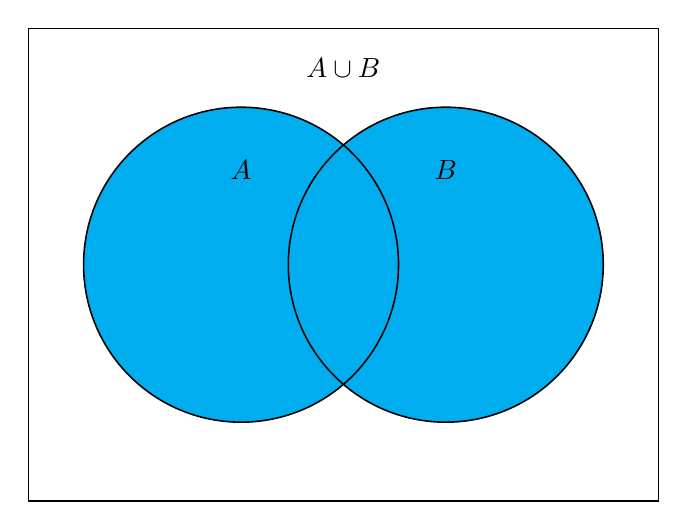
\begin{tikzpicture}[line width=0.2mm]

    % Coordinates for the centers of the circles.
    \coordinate (C1) at (-1.3, 0);
    \coordinate (C2) at ( 1.3, 0);

    % Coordinates for the labels.
    \coordinate (A) at (-1.3, 1.2);
    \coordinate (B) at ( 1.3, 1.2);
    \coordinate (U) at ( 0.0, 2.5);

    % Rectangle indicating the universe set.
    \draw (-4, -3) rectangle (4, 3);

    % Fill in the circle with cyan.
    \draw[fill=cyan, draw=none] (C1) circle (2);
    \draw[fill=cyan, draw=none] (C2) circle (2);

    % Give outlines to the circles.
    \draw (C1) circle (2);
    \draw (C2) circle (2);

    % Labels.
    \node at (A) {$A$};
    \node at (B) {$B$};
    \node at (U) {$A\cup{B}$};
\end{tikzpicture}
            \caption{The Union of Two Sets}
            \label{fig:Union_of_Two_Sets}
        \end{figure}
        \begin{lexample}{Union of Two Sets}{Union_of_Two_Sets}
            Let $A$ and $B$ be the sets defined by:
            \par\hfill\par
            \begin{subequations}
                \begin{minipage}[b]{0.49\textwidth}
                    \begin{equation}
                        A=\{\,a,\,b,\,c\,\}
                    \end{equation}
                \end{minipage}
                \hfill
                \begin{minipage}[b]{0.49\textwidth}
                    \begin{equation}
                        B=\{\,c,\,1,\,2\,\}
                    \end{equation}
                \end{minipage}
            \end{subequations}
            \par\vspace{2.5ex}
            The union of $A$ and $B$ is the set that contains all of the
            elements of $A$ and all of the elements of $B$, and only such
            elements. That is:
            \begin{equation}
                A\cup{B}=\{\,a,\,b,\,c,\,1,\,2\,\}
            \end{equation}
            Even though $c\in{A}$ and $c\in{B}$, $c$ only appears once in the
            union. This again because sets cannot account for repetition, so
            including $c$ twice would be redundant.
        \end{lexample}
        \begin{lexample}{More Unions of Two Sets}{More_Unions_of_Two_Set}
            Again using the notation found in Eqn.~\ref{eqn:Z_n_Ellipses},
            if we let $\mathbb{Z}_{n}$ denote the integers between $0$ and
            $n-1$, we have the following: If $n$ is less than $m$, then:
            \begin{equation}
                \mathbb{Z}_{n}\cup\mathbb{Z}_{m}=\mathbb{Z}_{m}
            \end{equation}
            This is because every element of $\mathbb{Z}_{n}$ is already
            and element of $\mathbb{Z}_{m}$, and thus taking the union adds
            nothing new to $\mathbb{Z}_{m}$, so the resulting set is
            $\mathbb{Z}_{m}$ itself. Again denoted the even and odd non-negative
            integers by $\mathbb{N}_{e}$ and $\mathbb{N}_{o}$, respectively,
            we see that:
            \begin{equation}
                \mathbb{N}_{e}\cup\mathbb{N}_{o}=\mathbb{N}
            \end{equation}
            This is because every non-negative integer $n\in\mathbb{N}$ is
            either even or odd, and thus either $n\in\mathbb{N}_{e}$ or
            $n\in\mathbb{N}_{o}$. Taking the union therefore gives the entire
            set $\mathbb{N}$. The union does not add anything more than
            $\mathbb{N}$ since $\mathbb{N}_{e}\subseteq\mathbb{N}$ and
            $\mathbb{N}_{o}\subseteq\mathbb{N}$.
        \end{lexample}
        We can combine the axiom schema of specification
        (Ax.~\ref{ax:Axiom_Schema_of_Specification}) with the existence of
        the union of two sets to define the intersection of two sets.
        \begin{fdefinition}{Intersection of Two Sets}{Intersection_of_Two_Sets}
            The intersection of two sets $A$ and $B$ is the set:
            \begin{equation}
                A\cap{B}=\{\,x\in{A}\cup{B}\;|\;a\in{A}\textrm{ and }b\in{B}\,\}
            \end{equation}
        \end{fdefinition}
        \begin{lexample}{Intersections of Two Sets}
                        {Intersections_of_Two_Sets}
            If we let $A$ and $B$ be the sets defined by:
            \par\hfill\par
            \begin{subequations}
                \begin{minipage}[b]{0.49\textwidth}
                    \begin{equation}
                        A=\{\,a,\,b,\,c\,\}
                    \end{equation}
                \end{minipage}
                \hfill
                \begin{minipage}[b]{0.49\textwidth}
                    \begin{equation}
                        B=\{\,c,\,1,\,2\,\}
                    \end{equation}
                \end{minipage}
            \end{subequations}
            \par\vspace{2.5ex}
            we have that the intersection is then:
            \begin{equation}
                A\cap{B}=\{\,1\,\}
            \end{equation}
            Furthermore, if we let $\mathbb{N}_{e}$ and $\mathbb{N}_{o}$ denote
            the even and odd non-negative integers, respectively, we have:
            \begin{equation}
                \mathbb{N}_{e}\cap\mathbb{N}_{o}=\emptyset
            \end{equation}
            This is precisely what was meant earlier when it was claimed that
            $\mathbb{N}_{e}$ and $\mathbb{N}_{o}$ are disjoint. If
            $n,m\in\mathbb{N}$ and if $n<m$, we have that:
            \begin{equation}
                \mathbb{Z}_{n}\cap\mathbb{Z}_{m}=\mathbb{Z}_{n}
            \end{equation}
            This is because every element of $\mathbb{Z}_{n}$ is an element
            of $\mathbb{Z}_{m}$. This creates a more general theorem that if
            $A\subseteq{B}$, then $A\cap{B}=A$. Intersections thus seem like
            antonyms of unions.
        \end{lexample}
        Similar to how the union of two sets can be visualized with Venn
        diagrams (Fig.~\ref{fig:Union_of_Two_Sets}), so can the intersection.
        \begin{figure}[H]
            \centering
            %--------------------------------Dependencies----------------------------------%
%   tikz                                                                       %
%-------------------------------Main Document----------------------------------%
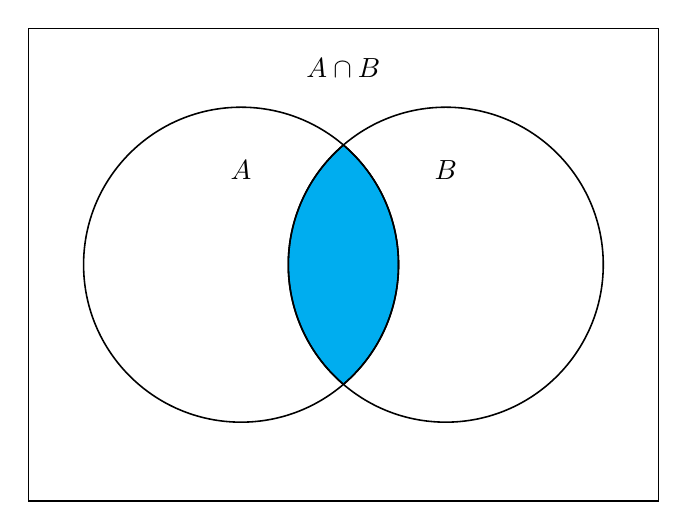
\begin{tikzpicture}[line width=0.2mm]
    % Coordinates for the centers of the circles.
    \coordinate (C1) at (-1.3, 0);
    \coordinate (C2) at ( 1.3, 0);

    % Coordinates for the labels.
    \coordinate (A) at (-1.3, 1.2);
    \coordinate (B) at ( 1.3, 1.2);
    \coordinate (I) at ( 0.0, 2.5);

    % Rectangle indicating the universe set.
    \draw (-4, -3) rectangle (4, 3);

    % Fill in the circle with cyan.
    \draw[fill=cyan] (0, -1.51987) arc(-49.46:49.46:2) arc(130.54:229.46:2);

    % Give outlines to the circles.
    \draw (C1) circle (2);
    \draw (C2) circle (2);

    % Labels.
    \node at (A) {$A$};
    \node at (B) {$B$};
    \node at (I) {$A\cap{B}$};
\end{tikzpicture}
            \caption{Venn Diagram for Intersection}
            \label{fig:Intersection_of_Two_Sets}
        \end{figure}
        We can extend this further and define the intersection over any
        collection of sets.
        \begin{fdefinition}{Intersection Over a Collection}
                           {Intersection_Over_a_Collection}
            The intersection over a set $\mathcal{O}$ of sets is the set:
            \begin{equation}
                \bigcap_{E\in\mathcal{O}}E
                =\Big\{\,x\in\bigcup_{E\in\mathcal{O}}\;|\;x\in{E}
                    \textrm{ for all }E\in\mathcal{O}\,\Big\}
            \end{equation}
        \end{fdefinition}
        Continuing in our goal of constructing order, we move on to the
        Cartesian product of two sets $A$ and $B$. This is the collection of
        all ordered pairs $(a,b)$ such that $a\in{A}$ and $b\in{B}$. To prove
        such a set exists required the \textit{axiom of the power set}.
        \begin{faxiom}{Axiom of the Power Set}{Axiom_of_the_Power_Set}
            If $X$ is a set, then there exists a set $\mathscr{P}$ such that,
            for all $A\subseteq{X}$, it is true that $A\in\mathscr{P}$.
        \end{faxiom}
        Again, much like the axiom of union and the axiom of pairing, this set
        may be bigger than we 
        \begin{theorem}
            \label{thm:Emptyset_Is_Subset}%
            If $A$ is a set, then $\emptyset\subseteq{A}$.
        \end{theorem}
        \begin{proof}
            For suppose not. Then there is an $x\in\emptyset$ such that
            $x\notin{A}$, a contradiction as for all $x$, it is true that
            $x\notin\emptyset$ (Def.~\ref{ax:Axiom_of_the_Empty_Set}).
            Therefore, etc.
        \end{proof}
        \begin{theorem}
            \label{thm:Subset_is_Transitive}%
            If $A$, $B$, and $C$ are sets, if $A\subseteq{B}$, and if
            $B\subseteq{C}$, then $A\subseteq{C}$.
        \end{theorem}
        \begin{proof}
            For suppose not. Then there is an $x\in{A}$ such that
            $x\notin{C}$. But $A$ is a subset of $B$ and thus $x\in{B}$
            (Def.~\ref{def:Subsets}). But $B$ is a subset of $C$ and
            therefore $x\in{C}$ (Def.~\ref{def:Subsets}). But $x\notin{C}$,
            a contradiction. Therefore, etc.
        \end{proof}
        \begin{theorem}
            \label{thm:Set_Is_Subset_Of_Self}%
            If $A$ is a set, then $A\subseteq{A}$.
        \end{theorem}
        \begin{proof}
            Suppose not. Then there is an $x\in{A}$
            such that $x\notin{A}$, a contradiction.
        \end{proof}
        It would be useful to distinguish between subsets that aren't the
        entire set.
        We write $A\ne{B}$ to denote that $A$ and $B$ are not equal sets.
        From the definition, we have inequality when either
        $A\nsubseteq{B}$ or $B\nsubseteq{A}$. We can now rigorously restate
        our claim that the empty set is unique.
        \begin{theorem}
            If $\emptyset'$ is a set with no elements,
            then $\emptyset=\emptyset'$.
        \end{theorem}
        \begin{proof}
            For suppose not. But $\emptyset'$ is a set, and thus
            $\emptyset\subseteq\emptyset'$
            (Thm.~\ref{thm:Emptyset_Is_Subset}). Therefore
            $\emptyset'\nsubseteq\emptyset$. But then there is an $x$ such
            that $x\in\emptyset'$ and $x\notin\emptyset$. But $\emptyset'$
            contains no elements, a contradiction. Thus
            $\emptyset'\subseteq\emptyset$. Therefore,
            $\emptyset=\emptyset'$ (Def.~\ref{def:Equal_Sets}).
        \end{proof}
        \begin{theorem}
            \label{thm:Subsets_of_Equal_Sets}%
            If $A$, $B$, and $C$ are sets, if $A=B$, and if
            $C\subseteq{A}$, then $C\subseteq{B}$.
        \end{theorem}
        \begin{proof}
            For if $A=B$, then $A\subseteq{B}$ (Def.~\ref{def:Equal_Sets}).
            But if $C\subseteq{A}$ and $A\subseteq{B}$, then $C\subseteq{B}$
            (Thm.~\ref{thm:Subset_is_Transitive}). Therefore, etc.
        \end{proof}
        \begin{theorem}
            \label{thm:Equality_Symmetric}%
            If $A$ and $B$ are equal sets, then $B$ and
            $A$ are equal sets.
        \end{theorem}
        \begin{proof}
            For suppose not. If $B\ne{A}$, then either
            $B\nsubseteq{A}$ or $A\nsubseteq{B}$.
            But $A=B$, and thus $A\subseteq{B}$  and
            $B\subseteq{A}$ (Def.~\ref{def:Equal_Sets}),
            a contradiction. Therefore, etc.
        \end{proof}
        \begin{theorem}
            \label{thm:Equality_Reflexive}%
            If $A$ is a set, then $A=A$.
        \end{theorem}
        \begin{proof}
            For if $A$ is a set then $A\subseteq{A}$
            (Thm.~\ref{thm:Set_Is_Subset_Of_Self}).
            Therefore, etc.
        \end{proof}
        \begin{theorem}
            \label{thm:Equality_Transitive}%
            If $A$, $B$, and $C$ are sets, if $A=B$, and if
            $B=C$, then $A=C$.
        \end{theorem}
        \begin{proof}
            For if $B=C$, then $C\subseteq{B}$
            (Def.~\ref{def:Equal_Sets}). But if
            $A=B$, then $B=A$
            (Thm.~\ref{thm:Equality_Symmetric}). But if
            $B=A$ and and $C\subseteq{B}$, then
            $C\subseteq{A}$
            (Thm.~\ref{thm:Subsets_of_Equal_Sets}).
            And if $A=B$, then $A\subseteq{B}$
            (Def.~\ref{def:Equal_Sets}). But if $B=C$ and
            $A\subseteq{B}$, then $A\subseteq{C}$
            (Thm.~\ref{thm:Subsets_of_Equal_Sets}). But it
            was just proved that $C\subseteq{A}$, and
            thus $A=C$ (Def.~\ref{def:Equal_Sets}).
            Therefore, etc.
        \end{proof}
        These three properties,
        Thms.~\ref{thm:Equality_Reflexive}-%
        \ref{thm:Equality_Transitive}, are the key ingredients to define
        \textit{equivalence relations}. We'll develop this later once
        we've discussed the notion of \textit{Cartesian Products}.
        But first, we now define what a proper subset is.
        \begin{theorem}
            \label{thm:Prop_Subset_Not_Equal}%
            If $A$ and $B$ are sets, and if $A$ is a proper
            subset of $B$, then there is an $x\in{B}$ such
            that $x\notin{A}$.
        \end{theorem}
        \begin{proof}
            For suppose not. Then for all $x\in{B}$,
            it is true that $x\in{A}$. But then
            $B$ is a subset of $A$ (Def.~\ref{def:Subsets}).
            But $A$ is a subset of $B$, and thus $A=B$
            (Def.~\ref{def:Equal_Sets}), a contradiction as
            $A$ is a proper subset. Therefore, etc.
        \end{proof}
        Theorem \ref{thm:Prop_Subset_Not_Equal} can
        be used as an equivalent definition of a proper
        subset. That is, a proper subset is a subset that
        is missing at least one element. The notation
        $\subseteq$ and $\subsetneq$ is analogous to the
        notation of inequalities that one finds in calculus,
        $\leq$ and $<$. In many texts, the two symbols
        $\subseteq$ and $\subset$ are taken to be identical,
        which can be a cause for confusion. In attempt to
        reduce confusion, $\subseteq$ will denote any subset,
        $\subsetneq$ denotes a proper subset, and the symbol
        $\subset$ will be avoided.
    \subsection{Operations on Sets}
        Similar to the arithmetic of real numbers, there
        are standard operations that can be performed on
        sets to obtain new sets. The four most common
        operations are union, intersection, set difference,
        and symmetric difference. Often the
        \textit{complement} of a set is discussed, but as
        we will see, this is just a specific case of set
        difference.
        Set operations are very algebraic, and it is often
        useful to build up several small tools to eventually
        prove larger theorems in a simple way. We wish to
        show that union is commutative and associative, and
        that there is an \textit{identity}.
        \begin{ltheorem}{Commutative Law of Unions}
              {Commutative_Law_of_Unions}
            If $A$ and $B$ are sets, then
            $A\cup{B}=B\cup{A}$.
        \end{ltheorem}
        \begin{proof}
            For if $x\in{A}\cup{B}$, then either $x\in{A}$
            or $x\in{B}$, or both
            (Def.~\ref{def:Union_of_Two_Sets}). But then either
            $x\in{B}$ or $x\in{A}$, or both, and therefore
            $x\in{B}\cup{A}$ (Def.~\ref{def:Union_of_Two_Sets}).
            But then for all $x\in{A}\cup{B}$ it is true that
            $x\in{B}\cup{A}$, and therefore
            $A\cup{B}\subseteq{B}\cup{A}$
            (Def.~\ref{def:Subsets}). Similarly,
            $B\cup{A}\subseteq{A}\cup{B}$, and thus
            $A\cup{B}=B\cup{A}$ (Def.~\ref{def:Equal_Sets}).
            Therefore, etc.
        \end{proof}
        When taking the union of two sets, we obtain a
        \textit{larger} set, in a sense. Again relying on
        the analogy of arithmetic, given two non-negative
        integers $a$ and $b$, it is true that $a\leq{a}+b$.
        Equality is obtained if and only if either $a$ or
        $b$ is equal to zero. As we will see, the empty set
        acts as the \textit{zero} of unions. Also, given
        three non-negative integers $a$, $b$, and $c$, if
        $b\leq{c}$, then $a+b\leq{a}+c$. A similar result
        will hold for sets and unions.
        \begin{theorem}
            \label{thm:Union_is_Bigger}%
            If $A$ and $B$ are sets, then
            $A\subseteq{A}\cup{B}$.
        \end{theorem}
        \begin{proof}
            For suppose not. Then there is an $x\in{A}$ such
            that $x\notin{A}\cup{B}$. But if $x\in{A}$, then
            $x\in{A}$ or $x\in{B}$ and thus $x\in{A}\cup{B}$
            (Def.~\ref{def:Union_of_Two_Sets}), a
            contradiction. Therefore, etc.
        \end{proof}
        \begin{theorem}
            \label{thm:Union_With_Lesser_Set}%
            If $A$, $B$, and $C$ are sets, and if
            $B\subseteq{C}$, then
            $A\cup{B}\subseteq{A}\cup{C}$.
        \end{theorem}
        \begin{proof}
            For if $x\in{A}\cup{B}$, then either $x\in{A}$,
            or $x\in{B}$, or both
            (Def.~\ref{def:Union_of_Two_Sets}). But $B$ is a
            subset of $C$, and therefore if $x\in{B}$, then
            $x\in{C}$ (Def.~\ref{def:Subsets}).
            Thus, if $x\in{A}$ or $x\in{B}$, then
            $x\in{A}$ or $x\in{C}$, and therefore
            $x\in{A}\cup{C}$ (Def.~\ref{def:Union_of_Two_Sets}).
            Thus, $A\cup{B}\subseteq{A}\cup{C}$
            (Def.~\ref{def:Subsets}). Therefore, etc.
        \end{proof}
        \begin{theorem}
            If $A$, $B$, $C$, and $D$ are sets, if
            $A\subseteq{C}$, and if $B\subseteq{D}$, then
            $A\cup{B}\subseteq{C}\cup{D}$.
        \end{theorem}
        \begin{proof}
            For if $B\subseteq{D}$, then
            $A\cup{B}\subseteq{A}\cup{D}$
            (Thm.~\ref{thm:Union_With_Lesser_Set}).
            But $A\cup{D}=D\cup{A}$
            (Thm.~\ref{thm:Commutative_Law_of_Unions}).
            But if $A\subseteq{C}$, then
            $D\cup{A}\subseteq{D}\cup{C}$
            (Thm.~\ref{thm:Union_With_Lesser_Set}). But
            $D\cup{C}=C\cup{D}$
            (Thm.~\ref{thm:Commutative_Law_of_Unions}).
            And if $A\cup{B}\subseteq{A}\cup{D}$ and
            $A\cup{D}\subseteq{C}\cup{D}$, then
            $A\cup{B}\subseteq{C}\cup{D}$
            (Thm.~\ref{thm:Subset_is_Transitive}).
            Therefore, etc.
        \end{proof}
        Taking the union of subsets is redundant, as we
        simply obtain the larger set. This starts to break
        down the analogy between sets and arithmetic, since
        there is only one \textit{zero}. That is, there is
        only one number $b$ such that $a+b=a$, and that is
        $b=0$. While any subset acts as a \textit{zero} of a
        given set, the empty set has the property that it
        acts as a zero for \textit{every} set. It is the only
        set with this property, and thus the analogy with
        arithmetic is restored.
        \begin{theorem}
            \label{thm:Union_With_Subset}%
            If $A$ and $B$ are sets, and if
            $A\subseteq{B}$, then $A\cup{B}=B$.
        \end{theorem}
        \begin{proof}
            For if $A$ and $B$ are sets, then
            $B\subseteq{A}\cup{B}$
            (Thm.~\ref{thm:Union_is_Bigger}).
            But if $A\subseteq{B}$, then for all $x\in{A}$,
            it is true that $x\in{B}$
            (Def.~\ref{def:Subsets}). Thus if $x\in{A}$ or if
            $x\in{B}$, then $x\in{B}$. But then, for all
            $x\in{A}\cup{B}$, it is true that $x\in{B}$, and
            therefore $A\cup{B}\subseteq{B}$
            (Def.~\ref{def:Subsets}). Thus,
            $A\cup{B}=B$ (Def.~\ref{def:Equal_Sets}).
            Therefore, etc.
        \end{proof}
        \begin{theorem}
            \label{thm:Union_with_Emptyset}%
            If $A$ is a set, then $A=\emptyset\cup{A}$.
        \end{theorem}
        \begin{proof}
            For $\emptyset\subseteq{A}$
            (Thm.~\ref{thm:Emptyset_Is_Subset}) and
            therefore $\emptyset\cup{A}=A$
            (Thm.~\ref{thm:Union_With_Subset}).
        \end{proof}
        \begin{theorem}
            \label{thm:Empty_Set_Is_Zero_for_Unions}%
            If $A$ is a set such that, for any set $B$, it is
            true that $A\cup{B}=B$, then $A$ is the
            empty set.
        \end{theorem}
        \begin{proof}
            For suppose not. If $A\ne\emptyset$, then there
            is an $x\in{A}$ (Def.~\ref{ax:Axiom_of_the_Empty_Set}).
            But then $B=\{A\}$ is a set
            (Def.~\ref{def:Sets}). But then $x\in{A}\cup{B}$
            (Def.~\ref{def:Union_of_Two_Sets}). But $x\notin{B}$,
            and thus $A\cup{B}\ne{B}$
            (Def.~\ref{def:Equal_Sets}), a contradiction
            since $A$ is such that for any set $B$, it is
            true that $A\cup{B}=B$. Therefore, etc.
        \end{proof}
        Thm.~\ref{thm:Empty_Set_Is_Zero_for_Unions} proves
        the assertion that the empty set is the zero of set
        union. The converse of
        Thm.~\ref{thm:Union_With_Subset} can be proved as
        well.
        \begin{theorem}
            \label{thm:Conv_Union_Is_Bigger}%
            If $A$ and $B$ are sets, and if
            $A\cup{B}\subseteq{A}$, then $A\cup{B}=A$.
        \end{theorem}
        \begin{proof}
            For $A\subseteq{A}\cup{B}$
            (Thm.~\ref{thm:Union_is_Bigger}). But by
            hypothesis, $A\cup{B}\subseteq{A}$. But then
            $A=A\cup{B}$ (Def.~\ref{def:Equal_Sets}).
            Therefore, etc.
        \end{proof}
        \begin{theorem}
            \label{thm:Union_is_Equal}%
            If $A$ and $B$ are sets, and if
            $A\cup{B}\subseteq{A}$, then $B\subseteq{A}$.
        \end{theorem}
        \begin{proof}
            For if $A\cup{B}\subseteq{A}$, then
            $A\cup{B}=A$
            (Thm.~\ref{thm:Conv_Union_Is_Bigger}). And also,
            $B\subseteq{A}\cup{B}$
            (Thm.~\ref{thm:Union_is_Bigger}). But if
            $A\cup{B}=A$ and $B\subseteq{A}\cup{B}$, then
            $B\subseteq{A}$
            (Thm.~\ref{thm:Subsets_of_Equal_Sets}).
            Therefore, etc.
        \end{proof}
        We'll wrap up unions by showing that the operation
        is associative. Once again relying on the analogy
        of arithmetic, given three real numbers $a$, $b$,
        and $c$, it is true that $a+(b+c)=(a+b)+c$. This
        is called the associative law of addition. Combining
        this law with the commutative law shows that the
        order in which three real numbers are added is
        irrelevant. Applying induction, we see that given
        any finite collection of real numbers, the order in
        which we add them is again irrelevant. The same holds
        true for the union of sets.
        \begin{theorem}
            \label{thm:First_Assoc_Law_Union}%
            If $A$, $B$, and $C$ are sets, then
            $A\cup(B\cup{C})\subseteq(A\cup{B})\cup{C}$.
        \end{theorem}
        \begin{proof}
            For $B\subseteq{A}\cup{B}$
            (Thm.~\ref{thm:Union_is_Bigger}), and thus
            $B\cup{C}\subseteq(A\cup{B})\cup{C}$
            (Thm.~\ref{thm:Union_With_Lesser_Set}). But then
            $A\cup(B\cup{C})\subseteq{A}%
             \cup((A\cup{B})\cup{C})$
            (Thm.~\ref{thm:Union_With_Lesser_Set}).
            But $A\subseteq{A}\cup{B}$ and
            $A\cup{B}\subseteq(A\cup{B})\cup{C}$
            (Thm.~\ref{thm:Union_is_Bigger}), and therefore
            $A\subseteq(A\cup{B})\cup{C}$
            (Thm.~\ref{thm:Subset_is_Transitive}). But then
            $(A\cup)B\cup{C}={A}\cup((A\cup{B})\cup{C})$
            (Thm.~\ref{thm:Union_With_Subset}). But it was
            proved that
            $A\cup(B\cup{C})\subseteq{A}%
             \cup((A\cup{B})\cup{C})$, and therefore
            $A\cup(B\cup{C})\subseteq(A\cup{B})\cup{C}$
            (Thm.~\ref{thm:Subsets_of_Equal_Sets}).
            Therefore, etc.
        \end{proof}
        \begin{ltheorem}{Associative Law of Unions}
              {Associative_Law_of_Unions}
            If $A$, $B$, and $C$ are sets, then
            $A\cup(B\cup{C})=(A\cup{B})\cup{C}$.
        \end{ltheorem}
        \begin{proof}
            For by the Commutative Law of Unions
            (Thm.~\ref{thm:Commutative_Law_of_Unions}),
            we have:
            \begin{equation}
                (A\cup{B})\cup{C}=C\cup(A\cup{B})
                                 =C\cup(B\cup{A})
            \end{equation}
            But $C\cup(B\cup{A})\subseteq(C\cup{B})\cup{A}$
            (Thm.~\ref{thm:First_Assoc_Law_Union}). Again by
            commutativity, we obtain:
            \begin{equation}
                (C\cup{B})\cup{A}=A\cup(C\cup{B})=A\cup(B\cup{C})
            \end{equation}
            Therefore,
            $(A\cup{B})\cup{C}\subseteq{A}\cup(B\cup{C})$.
            But $A\cup(B\cup{C})\subseteq(A\cup{B})\cup{C}$
            (Thm.~\ref{thm:First_Assoc_Law_Union}),
            and thus $A\cup(B\cup{C})=(A\cup{B})\cup{C}$
            (Def.~\ref{def:Equal_Sets}). Therefore, etc.
        \end{proof}
        \begin{theorem}
            \label{thm:Redundant_Union}%
            If $A$, $B$, and $C$ are sets and if $A\subseteq{B}$, then
            $A\cup(B\cup{C})=B\cup{C}$
        \end{theorem}
        \begin{proof}
            For $B\cup{C}\subseteq{A}\cup(B\cup{C})$
            (Thm.~\ref{thm:Union_is_Bigger}). But
            $A\cup(B\cup{C})=(A\cup{B})\cup{C}$
            (Thm.~\ref{thm:Associative_Law_of_Unions}).
            And since $A$ is a subset of $B$, $A\cup{B}=B$
            (Thm.~\ref{thm:Union_With_Subset}), and thus
            $(A\cup{B})\cup{C}=B\cup{C}$. Thus, $B\cup{C}=A\cup(B\cup{C})$
            (Thm.~\ref{thm:Equality_Transitive}). Therefore, etc.
        \end{proof}
        \begin{figure}[H]
            \centering
            \captionsetup{type=figure}
            \begin{subfigure}[b]{0.49\textwidth}
                \centering
                \documentclass[crop,class=article]{standalone}
%----------------------------Preamble-------------------------------%
\usepackage{tikz}                       % Drawing/graphing tools.
%--------------------------Main Document----------------------------%
\begin{document}
    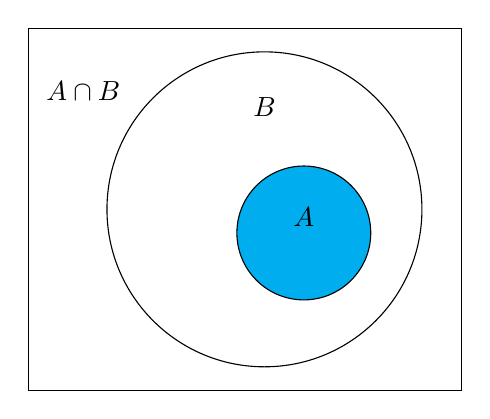
\begin{tikzpicture}
        \draw (-3,-2.3) rectangle (2.5,2.3);
        \draw (0,0) circle (2);
        \draw[fill=cyan] (0.5,-0.3) circle (0.85);
        \node at (0.5,-0.1) {$A$};
        \node at (0,1.3) {$B$};
        \node at (-2.3,1.5) {$A\cap{B}$};
    \end{tikzpicture}
\end{document}
                \subcaption{Visual for Thm.~\ref{thm:Intersection_of_Subset}.}
            \end{subfigure}
            \caption{Venn Diagrams for Intersections}
            \label{fig:Union_Intersection_venn_diagram}
        \end{figure}
        \begin{ltheorem}{Commutative Law of Intersections}{Commut_Law_Intersec}
            If $A$ and $B$ are sets, then $A\cap{B}=B\cap{A}$.
        \end{ltheorem}
        \begin{proof}
            For if $x\in{A}\cap{B}$, then $x\in{A}$ and
            $x\in{B}$. But then $x\in{B}$ and $x\in{A}$,
            and therefore $x\in{B}\cap{A}$
            (Def.~\ref{def:Intersection_of_Two}). But then
            for all $x\in{A}\cap{B}$ it is true that
            $x\in{B}\cap{A}$, and therefore
            $A\cup{B}\subseteq{B}\cup{A}$
            (Def.~\ref{def:Subsets}). Similarly,
            $B\cap{A}\subseteq{A}\cap{B}$, and thus
            $A\cap{B}=B\cap{A}$ (Def.~\ref{def:Equal_Sets}).
            Therefore, etc.
        \end{proof}
        \begin{theorem}
            \label{thm:Intersection_is_Smaller}%
            If $A$ snd $B$ are sets, then
            $A\cap{B}\subseteq{A}$.
        \end{theorem}
        \begin{proof}
            If $x\in{A}\cap{B}$, then $x\in{A}$ and
            $x\in{B}$, and thus $x\in{A}$. Therefore, etc.
        \end{proof}
        \begin{theorem}
            \label{thm:Intersection_with_Lesser_Set}%
            If $A$, $B$, and $C$ are sets, and if
            $B\subseteq{C}$, then
            $A\cap{B}\subseteq{A}\cap{C}$.
        \end{theorem}
        \begin{proof}
            For if $x\in{A}\cap{B}$, then $x\in{A}$ and
            $x\in{B}$ (Def.~\ref{def:Intersection_of_Two}).
            But $B$ is a subset of $C$, and thus if
            $x\in{B}$, then $x\in{C}$
            (Def.~\ref{def:Subsets}). But then $x\in{A}$ and
            $x\in{C}$, and therefore $x\in{A}\cap{C}$
            (Def.~\ref{def:Intersection_of_Two}). But
            then $A\cap{B}\subseteq{A}\cap{C}$
            (Def.~\ref{def:Subsets}). Therefore, etc.
        \end{proof}
        \begin{theorem}
            \label{thm:Intersection_is_Equal}%
            If $A$ and $B$ are sets, and if
            $A=A\cap{B}$, then $A\subseteq{B}$.
        \end{theorem}
        \begin{proof}
            For suppose not. Then there is an $x\in{A}$ such
            that $x\notin{B}$. But since $A=A\cap{B}$,
            if $x\in{A}$ then $x\in{A}\cap{B}$
            (Def.~\ref{def:Equal_Sets}). But if
            $x\in{A}\cap{B}$, then $x\in{B}$
            (Thm.~\ref{thm:Intersection_is_Smaller}),
            a contradiction. Therefore, etc.
        \end{proof}
        \begin{theorem}
            \label{thm:Intersection_of_Subset}%
            If $A$ and $B$ are sets, and if
            $A\subseteq{B}$, then $A\cap{B}=A$.
        \end{theorem}
        \begin{proof}
            For $A\cap{B}\subseteq{A}$
            (Thm.~\ref{thm:Intersection_is_Smaller}). But
            since $A$ is a subset of $B$, if $x\in{A}$, then
            $x\in{B}$ (Def.~\ref{def:Subsets}). But then
            $x\in{A}\cap{B}$
            (Def.~\ref{def:Intersection_of_Two}). Therefore,
            $A\subseteq{A}\cap{B}$ (Def~\ref{def:Subsets})
            and thus $A=A\cap{B}$ (Def~\ref{def:Equal_Sets}).
            Therefore, etc.
        \end{proof}
        \begin{theorem}
            \label{thm:Conv_Intersection_is_Smaller}%
            If $A$ and $B$ are sets, and if
            $A\subseteq{A}\cap{B}$, then $A=A\cap{B}$.
        \end{theorem}
        \begin{proof}
            For $A\cap{B}\subseteq{A}$
            (Thm.~\ref{thm:Intersection_is_Smaller}). But
            by hypothesis, $A\subseteq{A}\cap{B}$, and thus
            $A=A\cap{B}$ (Def.~\ref{def:Equal_Sets}).
            Therefore, etc.
        \end{proof}
        \begin{theorem}
            If $A$ is a set, then
            $\emptyset\cap{A}=\emptyset$.
        \end{theorem}
        \begin{proof}
            For $\emptyset\subseteq{A}$
            (Thm.~\ref{thm:Emptyset_Is_Subset}), and
            therefore $\emptyset\cap{A}=\emptyset$
            (Thm.~\ref{thm:Intersection_of_Subset}).
        \end{proof}
        \begin{theorem}
            \label{thm:First_Assoc_Law_Intersec}%
            If $A$, $B$, and $C$ are sets, then
            $A\cap(B\cap{C})\subseteq(A\cap{B})\cap{C}$.
        \end{theorem}
        \begin{proof}
            For if $x\in{A}\cap(B\cap{C})$, then $x\in{A}$
            and $x\in{B}\cap{C}$
            (Def.~\ref{def:Intersection_of_Two}). But if
            $x\in{B}\cap{C}$, then $x\in{B}$ and $x\in{C}$
            (Def.~\ref{def:Intersection_of_Two}). But then
            $x\in{A}$ and $x\in{B}$, and therefore
            $x\in{A}\cap{B}$
            (Def.~\ref{def:Intersection_of_Two}). But
            then $x\in{A}\cap{B}$ and $x\in{C}$, and
            therefore $x\in(A\cap{B})\cap{C}$
            (Def.~\ref{def:Intersection_of_Two}). Thus,
            $A\cap(B\cap{C})\subseteq(A\cap{B})\cap{C}$
            (Def.~\ref{def:Subsets}). Therefore, etc.
        \end{proof}
        \begin{ltheorem}{Associative Law of Intersections}
              {Assoc_Law_Intersec}
            If $A$, $B$, and $C$ are sets, then
            $A\cap(B\cap{C})=(A\cap{B})\cap{C}$.
        \end{ltheorem}
        \begin{proof}
            For by the Commutative Law of Intersections
            (Thm.~\ref{thm:Commut_Law_Intersec}),
            we have:
            \begin{equation}
                (A\cap{B})\cap{C}=C\cap(A\cap{B})
                                 =C\cap(B\cap{A})
            \end{equation}
            But $C\cap(B\cap{A})\subseteq(C\cap{B})\cap{A}$
            (Thm.~\ref{thm:First_Assoc_Law_Intersec}).
            Again by commutativity, we obtain:
            \begin{equation}
                (C\cap{B})\cap{A}=A\cap(C\cap{B})
                                 =A\cap(B\cap{C})
            \end{equation}
            Therefore,
            $(A\cap{B})\cap{C}\subseteq{A}\cap(B\cap{C})$.
            But $A\cap(B\cap{C})\subseteq(A\cap{B})\cap{C}$
            (Thm.~\ref{thm:First_Assoc_Law_Intersec}),
            and thus $A\cap(B\cap{C})=(A\cap{B})\cap{C}$
            (Def.~\ref{def:Equal_Sets}). Therefore, etc.
        \end{proof}
        \begin{theorem}
            \label{thm:Redundant_Intersection}%
            If $A$, $B$, and $C$ are sets and if
            $B\subseteq{A}$, then
            $A\cap(B\cap{C})=B\cap{C}$.
        \end{theorem}
        \begin{proof}
            For $A\cup(B\cup{C})\subseteq{B}\cup{C}$
            (Thm.~\ref{thm:Intersection_is_Smaller}). But
            $A\cap(B\cap{C})=(A\cap{B})\cap{C}$
            (Thm.~\ref{thm:Assoc_Law_Intersec}).
            And since $B$ is a subset of $A$,
            $A\cap{B}=A$
            (Thm.~\ref{thm:Intersection_of_Subset}),
            and thus $(A\cap{B})\cap{C}=B\cap{C}$. Thus,
            $B\cap{C}=A\cap(B\cap{C})$
            (Thm.~\ref{thm:Equality_Transitive}).
            Therefore, etc.
        \end{proof}
        \begin{theorem}
            \label{thm:First_Pseudo_Dist_Law_Union}%
            If $A$, $B$, and $C$ are sets, then
            $(B\cap{C})\subseteq(A\cup{B})\cap(A\cup{C})$.
        \end{theorem}
        \begin{proof}
            For $B\subseteq{A}\cup{B}$
            (Thm.~\ref{thm:Union_is_Bigger}). But then
            $B\cap{C}\subseteq(A\cup{B})\cap{C}$
            (Thm.~\ref{thm:Intersection_with_Lesser_Set}).
            But $C\subseteq{A}\cup{C}$
            (Thm.~\ref{thm:Union_is_Bigger}), and thus
            $(A\cup{B})\cap{C}%
             \subseteq(A\cup{B})\cap{A}\cup{C}$
            (Thm.~\ref{thm:Intersection_with_Lesser_Set}).
            But it was just proved that
            $B\cap{C}\subseteq(A\cup{B})\cap{C}$, and
            therefore by transivity,
            $(B\cap{C})\subseteq(A\cup{B})\cap(A\cup{C})$
            (Thm.~\ref{thm:Subset_is_Transitive}).
            Therefore, etc.
        \end{proof}
        \newpage
        \begin{ltheorem}{Distributive Law of Unions}
              {Distributive_Law_Union}
            If $A$, $B$, and $C$ are sets, then
            $A\cup(B\cap{C})=(A\cup{B})\cap(A\cup{C})$.
        \end{ltheorem}
        \begin{proof}
            For $(B\cap{C})\subseteq(A\cup{B})\cap(A\cup{C})$
            (Thm.~\ref{thm:First_Pseudo_Dist_Law_Union}).
            But then:
            \begin{equation}
                A\cup(B\cap{C})\subseteq
                A\cup\Big((A\cup{B})\cap(A\cup{C})\Big)
            \end{equation}
            But $A\cup((A\cup{B})\cap(A\cup{C}))%
                 =(A\cup{B})\cap(A\cup{C})$, and therefore:
            \begin{equation}
                A\cup(B\cap{C})\subseteq
                (A\cup{B})\cap(A\cup{C})
            \end{equation}
        \end{proof}
        \begin{ltheorem}{Distributive Law of Intersections}
              {Distributive_Law_Intersections}
            If $A$, $B$, and $C$ are sets, then
            $A\cap(B\cup{C})=(A\cap{B})\cup(A\cap{C})$.
        \end{ltheorem}
        \begin{proof}
            Hi
        \end{proof}
        If $A$ and $B$ are sets, and if
        $C\subseteq{A}\cup{B}$, then
        either $C\subseteq{A}$ or $C\subseteq{B}$, or both.
        It is possible that $C\subseteq{A}\cup{B}$ and yet
        $C$ and $B$ have no elements in common, as long
        as $C\subseteq{A}$. As an example,
        take $A$ and $B$ to be disjoint sets. Then
        $A\subseteq{A}\cup{B}$, yet $A$ and $B$ have no
        elements in common. If $C\subseteq{A}\cap{B}$, then
        it must be true that $C\subseteq{A}$ and
        $C\subseteq{B}$.
        Using arithmetic as an analogy, the empty set
        acts somewhat like a zero element. It is an identity
        element under set unions, and collapses everything
        down to zero under set intersections. Continuing
        with this analogy, we discuss set difference.
        \begin{ldefinition}{Set Difference}{Set_Difference}
            The set difference of a set $A$ with respect to
            a set $B$, denoted $B\setminus{A}$, is the set:
            \begin{equation}
                B\setminus{A}=\{x\in{B}:x\notin{A}\}
            \end{equation}
        \end{ldefinition}
        \begin{ldefinition}{Symmetric Difference}
              {Symmetric_Difference}
            The symmetric difference of $A$ and $B$, denoted
            $A\ominus{B}$, is the set:
            \begin{equation}
                A\ominus{B}
                =(A\cup{B})\setminus(A\cap{B})
            \end{equation}
        \end{ldefinition}
        While set difference appears similar to subtraction,
        the two have their differences. For any two real
        numbers $a$ and $b$, it is always true that
        $b=a-(a-b)$. For sets this is not true. For let $A$
        be the empty set, and let $B$ be non-empty.
        Then $A\setminus(A\setminus{B})=\emptyset$, which
        is not $B$. Set differences can not be easily
        simplified. The notion is not associative, nor is it
        commutative. If there is a larger \textit{universe}
        set, then set difference can be related to
        intersection.
        \begin{theorem}
            \label{thm:Set_Difference_As_Intersection}%
            If $A$, $B$, and $C$ are sets, and if
            $A\subseteq{C}$ and $B\subseteq{C}$, then:
            \begin{equation}
                B\setminus{A}=B\cap(C\setminus{A})
            \end{equation}
        \end{theorem}
        \begin{proof}
            For if $x\in{B}\setminus{A}$, then
            $x\in{B}$ and $x\notin{A}$. But
            $B\subseteq{C}$, and thus if $x\in{B}$, then
            $x\in{C}$. But if $x\notin{A}$, then
            $x\in{C}\setminus{A}$. Therefore
            $B\setminus{A}\subseteq{B}\cap(C\setminus{A})$.
            Similarly,
            $B\cap(C\setminus{A})\subseteq{B}\setminus{A}$,
            and therefore
            $B\setminus{A}={B}\cap(C\setminus{A})$.
        \end{proof}
        Similar to unions and intersections,
        set differences and symmetric differences can be
        visualized by Venn diagrams, as shown in
        Fig.~\ref{fig:Difference_Sym_Venn_Diagram}.
        \begin{figure}[H]
            \centering
            \captionsetup{type=figure}
            \begin{subfigure}[b]{0.49\textwidth}
                \centering
                %--------------------------------Dependencies----------------------------------%
%   tikz                                                                       %
%-------------------------------Main Document----------------------------------%
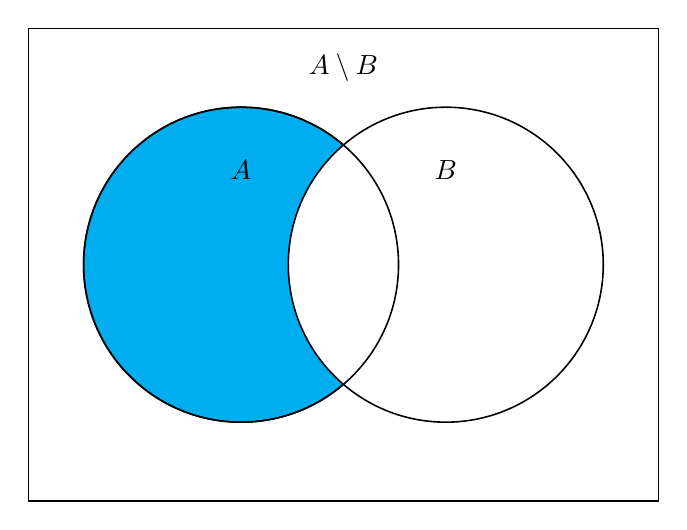
\begin{tikzpicture}[line width=0.2mm]

    % Coordinates for the centers of the circles.
    \coordinate (C1) at (-1.3, 0);
    \coordinate (C2) at ( 1.3, 0);

    % Coordinates for the labels.
    \coordinate (A) at (-1.3, 1.2);
    \coordinate (B) at ( 1.3, 1.2);
    \coordinate (U) at ( 0.0, 2.5);

    % Rectangle indicating the universe set.
    \draw (-4, -3) rectangle (4, 3);

    % Draw the two circles.
    \draw[fill=cyan]              (C1) circle (2);
    \draw[fill=white, draw=black] (C2) circle (2);

    % Add an outline to the left circle.
    \draw (C1) circle (2);

    % Labels.
    \node at (A) {$A$};
    \node at (B) {$B$};
    \node at (U) {$A\setminus{B}$};
\end{tikzpicture}
                \subcaption{Set Difference}
            \end{subfigure}
            \begin{subfigure}[b]{0.49\textwidth}
                \centering
                %--------------------------------Dependencies----------------------------------%
%   tikz                                                                       %
%-------------------------------Main Document----------------------------------%
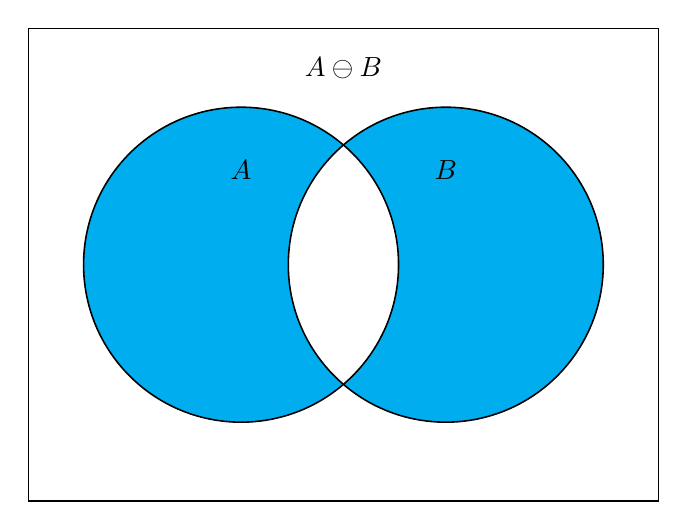
\begin{tikzpicture}[line width=0.2mm]

    % Coordinates for the centers of the circles.
    \coordinate (C1) at (-1.3, 0);
    \coordinate (C2) at ( 1.3, 0);

    % Coordinates for the labels.
    \coordinate (A) at (-1.3, 1.2);
    \coordinate (B) at ( 1.3, 1.2);
    \coordinate (S) at ( 0.0, 2.5);

    % Rectangle indicating the universe set.
    \draw (-4, -3) rectangle (4, 3);

    % Fill in the circle with cyan.
    \draw[fill=cyan, draw=none] (C1) circle (2);
    \draw[fill=cyan, draw=none] (C2) circle (2);

    % Fill in the circle with cyan.
    \draw[fill=white, draw=none] (0, -1.51987) arc(-49.46:49.46:2)
                                               arc(130.54:229.46:2);

    % Give outlines to the circles.
    \draw (C1) circle (2);
    \draw (C2) circle (2);

    % Labels.
    \node at (A) {$A$};
    \node at (B) {$B$};
    \node at (S) {$A\ominus{B}$};
\end{tikzpicture}
                \subcaption{Symmetric Difference}
            \end{subfigure}
            \caption[Venn Diagrams for Set Difference
                     and Symmetric Difference]
                    {Venn Diagrams Depicting the Set
                     Difference and Symmetric Difference
                     of the Sets $A$ and $B$.}
            \label{fig:Difference_Sym_Venn_Diagram}
        \end{figure}
        The concept of set difference can then be used to
        define the concept of complement.
        \begin{ldefinition}{Complement}{Complement}
            The complement of a set $A$ with respect to a set
            $\Omega$, denoted $A^{C}$, is the set:
            \begin{equation}
                A^{C}=\Omega\setminus{A}
            \end{equation}
        \end{ldefinition}
        Thm.~\ref{thm:Set_Difference_As_Intersection}
        can then be translated into the notation of
        complements as follows:
        \begin{theorem}
            If $A$, $B$, and $\Omega$ are sets,
            $A,B\subseteq\Omega$, and if $A^{C}$ is the
            complement of $A$ with respect to $\Omega$, then:
            \begin{equation}
                B\setminus{A}=B\cap{A}^{C}
            \end{equation}
        \end{theorem}
        \begin{proof}
            By the definition of complement,
            $A^{C}=\Omega\setminus{A}$.
            As $A\subseteq\Omega$ and $B\subseteq\Omega$, by
            Thm.~\ref{thm:Set_Difference_As_Intersection},
            $B\setminus{A}=B\cap(\Omega\setminus{A})$,
            and therefore $B\setminus{A}=B\cap{A}^{C}$.
        \end{proof}
        The main result about complements are known as
        DeMorgan's Laws. The laws relate unions and
        intersections by means of complements. The general
        laws hold for arbitrary unions and arbitrary
        intersections, as will be shown later.
        \begin{ftheorem}{DeMorgan's Laws}{MEASURE_DEMORGAN}
            If $A$, $B$, and $\Omega$ are sets, if
            $A\subseteq\Omega$ and $B\subseteq\Omega$, then:
            \begin{subequations}
                \begin{align}
                    \big(A\cap{B}\big)^{C}
                    &=A^{C}\cup{B}^{C}\\
                    \big(A\cup{B}\big)^{C}
                    &=A^{C}\cap{B}^{C}
                \end{align}
            \end{subequations}
        \end{ftheorem}
        With this, we can prove some results about
        set differences.
        \begin{theorem}
            If $A$ and $B$ are sets, then:
            \begin{equation}
                A=\big(A\cap{B}\big)
                    \cup\big(A\setminus{B}\big)
            \end{equation}
        \end{theorem}
        \begin{proof}
            For let $\Omega=A\cup{B}$. Then
            $A\subseteq\Omega$ and $B\subseteq\Omega$,
            and thus:
            \begin{subequations}
                \begin{align}
                    \big(A\cap{B})\cup\big(A\setminus{B}\big)
                    &=\big(A\cap{B}\big)
                        \cup\big(A\cap{B}^{C}\big)\\
                    &=A\cap(B\cup{B}^{C})\\
                    &=A\cap\Omega
                \end{align}
            \end{subequations}
            But by Thm.~\ref{thm:Intersection_is_Smaller},
            $A\cap\Omega=A$. Therefore, etc.
        \end{proof}
        \begin{theorem}
            If $A$, $B$, and $C$ are sets, then:
            \begin{equation}
                A\cap\big(B\setminus{C}\big)
                =\big(A\cap{B}\big)\cap\big(A\setminus{C}\big)
            \end{equation}
        \end{theorem}
        \begin{proof}
            For:
            \begin{subequations}
                \begin{align}
                    A\cap\big(B\setminus{C}\big)
                    &=A\cap\big(B\cap{C}^{C}\big)\\
                    &=\big(A\cap{A}\big)
                        \cap\big(B\cap{C}^{C}\big)\\
                    &=\big(A\cap{B}\big)
                        \cap\big(A\cap{C}^{C}\big)\\
                    &=\big(A\cap{B}\big)
                        \cap\big(A\setminus{C}\big)
                \end{align}
            \end{subequations}
        \end{proof}
        Intersections do distribute over set differences.
        \begin{theorem}
            If $A$, $B$, and $C$ are sets, then:
            \begin{equation}
                A\cap(B\setminus{C})=
                (A\cap{B})\setminus(A\cap{C})
            \end{equation}
        \end{theorem}
        \begin{proof}
            For:
            \begin{subequations}
                \begin{align}
                    \big(A\cap{B}\big)\setminus
                        \big(A\cap{C}\big)
                    &=\big(A\cap{B}\big)
                        \cap\big(A\cap{C}\big)^{C}\\
                    &=\big(A\cap{B}\big)
                        \cap\big(A^{C}\cup{C}^{C}\big)\\
                    &=\big[\big(A\cap{B}\big)\cap{A}^{C}\big]
                        \cup\big[\big({A}\cap{B}\big)
                        \cap{C}^{C}\big]\\
                    &=\big[\big(A\cap{A}^{C}\big)\cap{B}\big]
                        \cup\big[\big(A\cap{B}\big)
                        \cap{C}^{C}\big]\\
                    &=\emptyset\cup\big[\big(A\cap{B}\big)
                        \cap{C}^{C}\big]\\
                    &=\big(A\cap{B}\big)\cap{C}^{C}\\
                    &=A\cap\big(B\cap{C}^{C}\big)\\
                    &=A\cap\big(B\setminus{C}\big)
                \end{align}
            \end{subequations}
            Therefore, etc.
        \end{proof}
        Unions do not, however. For let $A$ be non-empty
        and let $A=B=C$. Then $A\cup(B\setminus{C})=A$, but
        $(A\cup{B})\setminus(A\cup{C})=\emptyset$.
        DeMorgan's Laws hold for arbitrary collections
        of set. If $I$ is some indexing set:
        \begin{align}
            \Big(\bigcup_{\alpha\in{I}}A_{\alpha}\Big)^{C}
            &=\bigcap_{\alpha\in{I}}A_{\alpha}^{C}\\
            \Big(\bigcap_{\alpha\in{I}}A_{\alpha}\Big)^{C}
            &=\bigcup_{\alpha\in{I}}A_{\alpha}^{C}
        \end{align}
        The set operations thus define binary operations
        on the power set of a set $\Omega$. It's important
        to note the notation. An element of $\Omega$ may
        be anything, while an element of
        $\mathcal{P}(\Omega)$ is a subset of $\Omega$.
        That is, the \textit{points} of $\mathcal{P}(\Omega)$
        are themselves sets. Thus, union, intersection,
        etc., define binary operations on
        $\mathcal{P}(\Omega)$. Given two subsets of
        $\Omega$, $A$ and $B$, $A\cup{B}$ is another
        subset of $\Omega$, as is $A\cap{B}$, and so on.
        The complement can also be seen as a unary operator
        on $\mathcal{P}(\Omega)$.
    \subsection{Cartesian Products}
        \begin{lexample}{The Cartesian Plane}{Cartesian_Plane}
            One example of a Cartesian product is the Euclidean plane,
            $\mathbb{R}^{2}$. This is the set:
            \begin{equation}
                \mathbb{R}^{2}=\mathbb{R}\times\mathbb{R}
            \end{equation}
            Where $\mathbb{R}$ denotes the set of real numbers.
            $\mathbb{R}^{2}$ is thus the set of all ordered pairs of real
            numbers. This is the same thing as the \textit{Cartesian}
            plane. Points in the Cartesian plane are identified by their
            \textit{coordinates}, $P=(x,y)$.
        \end{lexample}
        \begin{lexample}{}{Basic_Cartesian_Products}
            For the sake of computation, consider the set $A=\{1,2,3\}$ and
            $B=\{a,b\}$. We can then compute $A\times{B}$ directly:
            \begin{equation}
                A\times{B}=\big\{(1,a),(1,b),(2,a),(2,b),(3,a),(3,b)\big\}
            \end{equation}
            We can also compute $A\times{A}$ and $B\times{B}$:
            \begin{subequations}
                \begin{align}
                    A\times{A}&=\big\{(1,1),(1,2),(1,3),
                                      (2,1),(2,2),(2,3),
                                      (3,1),(3,2),(3,3)\big\}\\
                    B\times{B}&=\big\{(a,a),(a,b),(b,a),(b,b)\big\}
                \end{align}
            \end{subequations}
            Lastly, compute $B\times{A}$:
            \begin{equation}
                B\times{A}=\big\{
                    (a,1),(a,2),(a,3),
                    (b,1),(b,2),(b,3)\big\}
            \end{equation}
            Note that, since for distinct elements $\alpha$
            and $\beta$, we have that
            $(\alpha,\beta)\ne(\beta,\alpha)$, and thus
            the Cartesian products $A\times{B}$ and $B\times{A}$
            are not equal, in general. Equality is obtained
            if and only if $A=B$.
        \end{lexample}
        Note that in
        Ex.~\ref{ex:Basic_Cartesian_Products}, the
        \textit{size} of the Cartesian product of two sets
        was simply the product of the number of elements of
        the constituent sets. That is, we see that $A$ has
        three elements and $B$ has two elements, but also that
        $A\times{B}$ has six elements. Moreover, $A\times{A}$
        has nine elements, and $B\times{B}$ has four. This
        pattern holds for \textit{finite} sets. To be precise,
        we need to define what finite sets are, and what
        are \textit{infinite} sets. To do this we need the
        notion of a function.
    \subsection{Definitions}
        Given two sets $A$ and $B$, and a function
        $f:A\rightarrow{B}$, we often call $A$ the
        domain of $f$ and $B$ the co-domain.
        The \textit{image} of $x\in{X}$ is often written
        as $y=f(x)$. Requiring that $y$ be unique for each
        $x$ is equivalent to the \textit{vertical line test}
        one might find in a calculus course. We can also
        define the image of a subset of $Y$.
        \begin{ldefinition}{Image of a Set}
              {Funct_Analysis_Image_of_Set}
            The \gls{set image} of a subset
            $S\subseteq{X}$ by a function
            $f:X\rightarrow{Y}$ is the set:
            \begin{equation}
                f(S)=\{f(x)\in{Y}:x\in{X}\}
            \end{equation}
            That is, the set of all points in $Y$ that $S$
            gets mapped to by $f$.
        \end{ldefinition}
        This is also called the \textit{range} of a function.
        In a similar manner, we can define the pre-image, or
        inverse image, of a set.
        \begin{ldefinition}{Pre-Image of a Set}
              {Funct_Analysis_Pre_Image_of_Set}
            The \gls{pre-image} of $S\subseteq{Y}$
            by a function $f:X\rightarrow{Y}$ is the set:
            \begin{equation}
                f^{\minus{1}}(S)=\{x\in{X}:f(x)\in{S}\}
            \end{equation}
            That is, the set of all points in $X$ that map
            into $S$.
        \end{ldefinition}
        \begin{lexample}{}{Image_Is_Non_Empty}
            Given a function $f:X\rightarrow{Y}$, and any non-empty subset
            $S\subseteq{X}$, the image $f(S)$ is non-empty. This is not
            true for the pre-image of a function. For let
            $f:\mathbb{R}\rightarrow\mathbb{R}$ be defined by $f(x)=1$ for
            all $x\in\mathbb{R}$. Then, for any subset $S\subset\mathbb{R}$
            such that $1\notin{S}$, we have that
            $f^{\minus{1}}(S)=\emptyset$.
        \end{lexample}
        There are many examples of functions, but certain ones are easier
        to study than others. We give some of these special functions names.
        \begin{ldefinition}{Injective Functions}{Injective_Function}
            An \gls{injective function} is a function
            $f:X\rightarrow{Y}$ such that, for all
            $x,y\in{X}$ such that $x\ne{y}$, it is true that
            $f(x)\ne{f}(y)$.
        \end{ldefinition}
        That is, an injective function is a function
        $f:X\rightarrow{Y}$ such that $f(x_{1})=f(x_{2})$
        if and only if $x_{1}=x_{2}$. Such functions are also
        called \textit{one-to-one}.
        \begin{lexample}{}{Natural_Log_Is_Injective}
            Consider the natural logarithm
            $\ln:\mathbb{R}^{+}\rightarrow\mathbb{R}$. This is an injective
            function. For let $x,y\in\mathbb{R}^{+}$ be such that
            $x\ne{y}$. Suppose $\ln(x)=\ln(y)$. But then:
            \begin{equation}
                \ln(x)-\ln(y)=\ln\Big(\frac{x}{y}\Big)=0
            \end{equation}
            Recall the definition of the natural logarithm:
            \begin{equation}
                \ln(t)=\int_{1}^{t}\frac{1}{x}\diff{x}
            \end{equation}
            But then $\ln(t)=0$ if and only if $t=1$. Thus $x=y$, a
            contradiction. Therefore $\ln$ is an injective function. Not
            every function is injective, for define
            $f:\mathbb{R}\rightarrow\mathbb{R}$ by $f(x)=x^{2}$. Then, for
            all $x\in\mathbb{R}^{+}$, $f(\minus{x})=f(x)$, and thus $f$
            cannot be an injective function.
        \end{lexample}
        One might think that most functions are not injective,
        and indeed for the \textit{finite} case, this is true.
        For let $A$ and $B$ be finite sets with $n$ and $m$
        elements, respectively. If $m<n$, there can't be
        any injective function. Consider the case when $n=m$.
        Then we are simply counting the number of ways to
        permute the elements of $A$. This is $n!$. On the
        other hand, the total number of functions is
        $n^{n}$. Thus, the ratio of the number of injective
        functions to the number of functions is
        $n!/n^{n}$, and this decays to zero rapidly as
        $n$ get's large. Finally, if $m>n$, then the total
        number of injective functions is
        $n!\binom{m}{n}$, where $\binom{m}{n}$ is the
        binomial coefficient. The total number of functions
        is $n^{m}$. The ratio is thus:
        \begin{equation}
            \frac{n!\binom{m}{n}}{n^{m}}=\frac{n!\frac{m!}{n!(m-n)!}}{n^{m}}
                                        =\frac{m!}{(m-n)!n^{m}}
        \end{equation}
        And again, this decays rapidly to zero and $n$ and $m$
        get large. Later, when we define infinite sets
        and the notion of Cardinality, we'll show that this
        trend continues. That is, in a sense, \textit{most}
        functions from a set $A$ to a sufficiently large set
        $B$ are not injective. Next, we define
        \textit{surjective} functions.
        \begin{ldefinition}{Surjective Functions}{Surjective_Function}
            A \gls{surjective function} is a function
            $f:X\rightarrow{Y}$ such that $f(X)=Y$.
            That is, for all $y\in{Y}$, there is an
            $x\in{X}$ such that $f(x)=y$.
        \end{ldefinition}
        That is, every point $y\in{Y}$ gets mapped to by
        at least one point in $X$. It may also be true that
        many points in $X$ map to the same point in $Y$.
        The notions of surjective functions and injective
        functions are distinct, and neither implies the
        other. Surjective functions are also called
        \textit{onto}.
        \begin{ldefinition}{Bijective Functions}{Bijective_Function}
            A \gls{bijective function} is a function
            that is both injective and surjective.
        \end{ldefinition}
        Sets $X$ and $Y$ such that there exists a bijective function
        $f:X\rightarrow{Y}$ are called \textit{equivalent}. Such sets can
        be said to have the same size. We say that $X$ is strictly
        smaller than $Y$ if there is an injective function
        $f:X\rightarrow{Y}$, but no bijective function.
        \begin{definition}
            A finite set is a set $X$ such that there exists an
            $n\in\mathbb{N}$ such that there is a bijective function
            $f:\mathbb{Z}_{n}\rightarrow{S}$
        \end{definition}
        \begin{definition}
            A countable set is a set $X$ such that there exists a
            bijective function $f:\mathbb{N}\rightarrow{X}$.
        \end{definition}
        Being countable means you can write
        the elements out in a list, or a
        one-to-one correspondence with all of
        the positive integers. Many sets are countable,
        including the whole numbers, integers, rational
        numbers, and \textit{algebraic} numbers. The
        union of finitely many countable sets is also
        countable, as is the union of countably many
        countable sets.
        \begin{example}
            The set of all positive even integers is
            countable. For let $\mathbb{N}_{e}$ be the
            set of all even integers and define
            $f:\mathbb{N}\rightarrow\mathbb{N}_{e}$ be
            $f(n)=2n$ for all $n\in\mathbb{N}$. This is
            a bijection, and thus $\mathbb{N}_{e}$ is
            countable. The set of all odd positive integers
            is countable, as shown by letting
            $f(n)=2n-1$. Even though the set of even
            integers may seem ``smaller,'' than the set of
            all integers, they are equivalent. The set of
            all integers $\mathbb{Z}$ is also countable.
            For let $f:\mathbb{N}\rightarrow\mathbb{Z}$
            be defined as:
            \begin{equation}
                f(n)=
                \begin{cases}
                    \frac{1}{2}(n-1),&n\textrm{ odd}\\
                    -\frac{n}{2},&n\textrm{ even}
                \end{cases}
            \end{equation}
        \end{example}
        Any set that is infinite (Not finite) contains a
        countable subset. Thus, $\mathbb{N}$ can be
        considered as the \textit{smallest} infinite set.
        \begin{theorem}
            If $A$ is an infinite set, then there exists
            $S\subseteq{A}$ such that $S$ is countabl e.
        \end{theorem}
        \begin{proof}
            For as $A$ is infinite, for all $n\in\mathbb{N}$
            there exists a set $B\subseteq{A}$ such that
            $|B|=n$. For all $n\in\mathbb{N}$,
            define the following:
            \begin{equation}
                \mathcal{S}_{n}=\{B\subseteq{A}:|B|=n\}
            \end{equation}
            Let $\mathcal{S}$ be defined as:
            \begin{equation}
                \mathcal{S}=\{\mathcal{S}_{n}:n\in\mathbb{N}\}
            \end{equation}
            Then $\mathcal{S}$ is countable, for
            $a:\mathbb{N}\rightarrow\mathcal{S}$ defined
            by $a_{n}=\mathcal{S}_{n}$ is a bijection.
            By the axiom of choice, there is a function:
            \begin{equation}
                \alpha:\mathcal{S}\rightarrow
                \bigcup_{n=1}^{\infty}\mathcal{S}_{n}
            \end{equation}
            Such that, for all $x\in\mathcal{S}$,
            $\alpha(x)\in{x}$. But then, for all
            $x\in\mathcal{S}$, $\alpha(x)$ is a subset
            of $A$. But for all $x\in\mathcal{S}$, there
            is an $n\in\mathbb{N}$ such that
            $a_{n}=x$. Thus, let $S$ be the following:
            \begin{equation}
                S=\bigcup_{n=1}^{\infty}\alpha(a_{n})
            \end{equation}
        \end{proof}
        \begin{theorem}
            \label{thm:Funct_Countable_Union_of_Countable}
            If $A$ is a countable set such that for all
            $\mathcal{U}\in{A}$, $\mathcal{U}$ is a
            countable set, and if for all $a,b\in{A}$,
            $a\cap{b}=\emptyset$, then
            $\bigcup_{\mathcal{U}\in{A}}\mathcal{U}$
            is countable set.
        \end{theorem}
        \textit{Sketch of Proof.} The proof of
        Thm.~\ref{thm:Funct_Countable_Union_of_Countable}
        follows in the same manner
        as proving that the rationals are countable. Since
        there are countably many sets, write them out in
        a list $\mathcal{U}_{1}$, $\mathcal{U}_{2}$, and
        so on. Then write out the elements in a table as
        follows:
        \begin{table}[H]
            \captionsetup{type=table}
            \centering
            \begin{tabular}{ccccc}
                $u_{11}$&$u_{12}$&$u_{13}$
                &$u_{14}$&$\hdots$\\
                $u_{21}$&$u_{22}$&$u_{23}$
                &$u_{24}$&$\hdots$\\
                $u_{31}$&$u_{32}$&$u_{33}$
                &$u_{34}$&$\hdots$\\
                $u_{41}$&$u_{42}$&$u_{43}$
                &$u_{44}$&$\hdots$\\
                $\vdots$&$\vdots$&$\vdots$
                &$\vdots$&$\ddots$
            \end{tabular}
            \caption{Construction of a Bijection on the
                     Countable Union of Countably Infinite
                     Sets.}
            \label{table:Func_Countable_Union_of_Countable}
        \end{table}
        Where $u_{nm}$ is the $m^{th}$ element of
        $\mathcal{U}_{n}$.
        Using the \textit{diagonal argument},
        we obtain:
        \begin{table}[H]
            \captionsetup{type=table}
            \centering
            \begin{tabular}{|c|c|c|c|c|c|c|c|c|c|c|}
                \hline
                $\mathbb{N}$&1&2&3&4&5&6&7&8&9&$\hdots$\\
                \hline
                $\bigcup_{\mathcal{U}\in{A}}\mathcal{U}$&
                $u_{11}$&$u_{12}$&$u_{21}$&$u_{13}$&
                $u_{22}$&$u_{31}$&$u_{14}$&$u_{23}$&
                $u_{32}$&$\hdots$\\
                \hline
            \end{tabular}
            \caption{The Bijection Between $\mathbb{N}$ and
                     $\bigcup_{\mathcal{U}\in{A}}\mathcal{U}$}
            \label{table:Func_Bijection_on_Countable_Union}
        \end{table}
        In the absence of the requirement that
        $a\cap{b}=\emptyset$ for all pairs in $\mathcal{U}$,
        we still have that the union is, at most, countable.
        The mapping we found would be a
        \textit{surjection}, rather than a bijection.
        The union is then either finite or countable. The
        Cantor-Schr\"{o}der-Bernstein Theorem can often be
        used to help identify the size of a set. This says
        that if $A$ and $B$ are sets such that there exists
        a surjective function $f:A\rightarrow{B}$ and a
        surjective function $g:B\rightarrow{A}$, then there
        is a bijective function $h:A\rightarrow{B}$. The
        requirement that $f$ and $g$ both be surjective
        can be replaced with the requirement that they both
        be injective. This is similar to saying that if
        $\Card(A)\leq\Card(B)$ and $\Card(B)\leq\Card(A)$,
        then $\Card(A)=\Card(B)$. Here, $\Card(A)$ denotes
        the \textit{cardinality} of the set $A$.
        \par\hfill\par
        \vspace{-2ex}
        For a set $X$, we often write
        $\mathcal{P}(X)$ to denote the
        \textit{power set} of $X$. This is the
        set of all subsets of $X$.
        For any set $X$ you can show that $X$ is
        strictly smaller than $\mathcal{P}(X)$.
        For example, $\mathcal{P}(\mathbb{N})$
        can be shown to be equivalent to $\mathbb{R}$.
        Since $\mathbb{N}$ is stricly smaller than
        $\mathbb{R}$, one might ask if there exists
        a set $X$ such that $\mathbb{N}$ is strictly
        smaller than $X$, but $X$ is strictly smaller
        than $\mathbb{R}$. Continuing, you can ask the
        same thing about $\mathbb{R}$ and
        $\mathcal{P}(\mathbb{R})$, and so on.
        This is called the continuum hypothesis.
        It turns out to be independent of
        the standard axioms of mathematics.
    \subsection{The Axiom of Choice}
        A relation on a set $X$ is a subset
        $R\subseteq{X}\times{X}$. Given an element
        $(x,y)\in{R}$, we often write $xRy$ to denote this.
        Here we'll write $x\leq{y}$.
        \begin{ldefinition}{Ordered Sets}
              {Funct_Analysis_Ordered_Set}
            An ordered set is a set $X$ and a relation
            $\leq$ on $X$, denoted $(X,\leq)$ such that
            the following are true:
            \begin{enumerate}
                \item For all $x\in{X}$, $x\leq{x}$.
                \item For all $x,y\in{X}$ such that $x\leq{y}$ and
                      $y\leq{x}$, it is true that $x=y$.
                \item For all $x,y,z\in{X}$ such that $x\leq{y}$
                      and $y\leq{z}$, it is true that $x\leq{z}$.
            \end{enumerate}
        \end{ldefinition}
        \begin{ldefinition}{Majorants in Ordered Sets}
              {Funct_Analysis_Majorant_in_Ord_Set}
            A majorant of a subset $Y\subseteq{X}$ of
            and ordered set $(X,\leq)$ is an element $x\in{X}$
            such that, for all $y\in{Y}$, it is true that
            $y\leq{x}$.
        \end{ldefinition}
        \begin{lexample}{}{}
            Let $(X,d)$ be a metric space, and let
            $x_{0}\in{X}$. Define the following:
            \begin{equation}
                \mathscr{N}(x_{0})=
                \big\{\mathcal{V}\subseteq{X}:\mathcal{V}
                    \textrm{ is a neighborhood of $x_{0}$}\big\}
            \end{equation}
            We can order $\mathscr{N}$ by reverse containment.
            That is, We have the following relation:
            \begin{equation}
                \leq=\big\{(\mathcal{U},\mathcal{V})\in
                    \mathscr{N}(x_{0})\times\mathscr{N}(x_{0})
                    :\mathcal{V}\subseteq\mathcal{U}\big\}
            \end{equation}
            That is, we write $\mathcal{U}\leq\mathcal{V}$ if
            $\mathcal{V}$ is a subset of $\mathcal{U}$. Note
            that, for all $x_{0}$,
            $\mathscr{x_{0}}$ has a least element, or a minorant,
            but $X$ is such an element. But, if $\{x_{0}\}$ is
            not open, then there is no majorant.
        \end{lexample}
        \begin{ldefinition}{Totally Ordered Sets}
              {Funct_Analysis_Tot_Ord_Set}
            A totally ordered set is an ordered set
            $(X,\leq)$ such that, for all $x,y\in{X}$, either
            $x\leq{y}$ or $y\leq{x}$.
        \end{ldefinition}
        \begin{ldefinition}{Maximal Element}
              {Funct_Analysis_Maximal_Element}
            A maximal element of a subset $Y\subseteq{X}$ of
            a totally ordered set $(X,\leq)$ is an element $y$
            such that:
            \begin{equation}
                \{y'\in{Y}:y\leq{y}'\}=\{y\}
            \end{equation}
            Note that $y$ is not necessary a majorant for $Y$
            nor is $y$ necessarily unique.
        \end{ldefinition}
        \begin{ldefinition}{Inductively Ordered Sets}
              {Funct_Analysis_Induct_Ordered_Set}
            An inductively ordered set is an ordered set
            $)X,\leq)$ such that, for all totally ordered
            subsets $S\subseteq{X}$, there is a majorant
            $x\in{X}$ of $S$.
        \end{ldefinition}
        That is, there exists $x\in{X}$ such that, for all
        $y\in{S}$, $y\leq{x}$.
        \begin{lexample}
            Let $X=\mathbb{R}$ and consider the set
            $\mathscr{N}(0)$. Then $\mathscr{N}(0)$ is
            not inductively ordered.
        \end{lexample}
        \begin{ltheorem}{Zorn's Lemma}
              {Funct_Analysis_Zorns_Lemma}
            If $(X,\leq)$ is an inductively ordered set,
            then there is a maximal element $x\in{X}$.
        \end{ltheorem}
    \subsection{Cardinality}
        We begin by talking about cardinality. This is the
        \textit{size} of a set. For an infinite set it
        doesn't make sense to talk about the \textit{number}
        of elements, but we can specify what it means two
        sets to have the same size.
        \begin{ldefinition}{Equivalent Sets}{Equivalent_Sets}
            Equivalent sets are set $A$ and $B$ such that
            there exists a bijection $f:A\rightarrow{B}$.
        \end{ldefinition}
        The notion of equivalent sets defines an equivalence
        relation on sets. That is, the notion is reflexive,
        symmetric, and transitive.
        \begin{theorem}
            If $A$ is a set, then $A$ is equivalent to $A$.
        \end{theorem}
        \begin{proof}
            For let $\mathrm{id}_{A}:A\rightarrow{A}$
            be the identity mapping, $\mathrm{id}_{A}(x)=x$,
            then $\mathrm{id}_{A}$ is a bijection, and thus
            $A$ is equivalent to $A$.
        \end{proof}
        \begin{theorem}
            If $A$ and $B$ are sets and if $A$ is equivalent
            to $B$, then $B$ is equivalent to $A$.
        \end{theorem}
        \begin{proof}
            For if $A$ is equivalent to $B$, then there is
            a bijection $f:A\rightarrow{B}$. But if $f$ is a
            bijection, then the inverse function
            $f^{-1}:B\rightarrow{A}$ is well-defined and is
            a bijection. Thus $B$ is equivalent to $A$.
        \end{proof}
        \begin{theorem}
            If $A$, $B$, and $C$ are sets, if $A$ is
            equivalent to $B$, and if $B$ is equivalent to
            $C$, then $A$ is equivalent to $C$.
        \end{theorem}
        \begin{proof}
            For if $A$ is equivalent to $B$, then there is
            a bijection $f:A\rightarrow{B}$. But if $B$ is
            equivalent ot $C$, then there is a bijection
            $g:B\rightarrow{C}$. But then
            $g\circ{f}:A\rightarrow{C}$ is a bijection, and
            thus $A$ and $C$ are equivalent.
        \end{proof}
        A bijection is a function that is both injective and
        surjective. Thus, two equivalent sets can be put
        into a one-to-one correspondence and can be said to
        have the same size. We then say that $A$ and $B$
        have the same cardinality. The notation is written
        as $|A|=|B|$ or $\Card(A)=\Card(B)$. Cardinality
        splits sets into one of three categories.
        \begin{ldefinition}{Finite Sets}{Finite_Sets}
            A finite set is a set $A$ such that there exists
            an $n\in\mathbb{N}$ such that there is a
            bijection $f:\mathbb{Z}_{n}\rightarrow{A}$, or
            such that $A=\emptyset$.
        \end{ldefinition}
        Sets that are not finite are called infinite. There
        are two types of infinite sets. Let $\mathbb{N}$
        denote the set of positive integers, or
        \textit{natural} numbers.
        \begin{ldefinition}{Countably Infinite Sets}
              {Countably_Infinite}
            A countably infinite set is a set $A$ such that
            is a bijection $f:\mathbb{N}\rightarrow{A}$.
        \end{ldefinition}
        Combining the notions of finite sets and countably
        infinite sets, we get the notion of
        \textit{countable} sets.
        \begin{ldefinition}{Countable Sets}
              {Countable_Sets}
            A countable set is a set $A$ such that $A$ is
            either finite or countably infinite.
        \end{ldefinition}
        Countable sets are also called \textit{listable}.
        This is because if $A$ is a countably infinite set,
        and if $a:\mathbb{N}\rightarrow{A}$ is a bijection,
        we can write $A$ as:
        \begin{equation}
            A=\{\;a_{n}\,:\,n\in\mathbb{N}\;\}
            =\{\,a_{1},\,a_{2},\,\dots,\,a_{k},\,\dots\,\}
        \end{equation}
        If $A$ is finite, and if
        $a:\mathbb{Z}_{n}\rightarrow{A}$ is a
        bijection, then we can write:
        \begin{equation}
            A=\{\;a_{n}\,:\,n\in\mathbb{Z}_{n}\;\}
             =\{\,a_{1},\,\dots,\,a_{n}\,\}
        \end{equation}
        Recall that functions $a:\mathbb{N}\rightarrow{A}$
        are called \textit{sequences}, and the image of
        $n\in\mathbb{N}$ is written $a_{n}$, rather than
        $a(n)$.
        \begin{lexample}{Countable Sets}{Countable_Sets}
            There are many commonly discussed sets that are
            countably infinite. $\mathbb{N}$ is a trivial
            such example, but also $\mathbb{N}_{e}$ and
            $\mathbb{N}_{o}$, the sets of even and odd
            positive integers, respectively. For consider as
            bijections the following functions:
            \par
            \begin{subequations}
                \begin{minipage}[b]{0.49\textwidth}
                    \centering
                    \begin{equation}
                        f_{e}(n)=2n
                    \end{equation}
                \end{minipage}
                \hfill
                \begin{minipage}[b]{0.49\textwidth}
                    \centering
                    \begin{equation}
                        f_{0}(n)=2n-1
                    \end{equation}
                \end{minipage}
                \par\vspace{2.5ex}
                The set of all integers, $\mathbb{Z}$ is also
                countable, as shown in
                Fig.~\ref{fig:Bijection_N_and_Z}.
                One bijection is:
                \begin{equation}
                    f(n)=
                    \begin{cases}
                        \frac{n}{2},&n\mod{2}=0\\
                        \frac{1-n}{2},&n\mod{2}=1
                    \end{cases}
                \end{equation}
            \end{subequations}
            Any subset of $\mathbb{Z}$ is countable,
            and this is true of any countable set.
        \end{lexample}
        \begin{figure}[H]
            \centering
            \captionsetup{type=figure}
            \documentclass[crop,class=article]{standalone}
%----------------------------Preamble-------------------------------%
\usepackage{tikz}
\usepackage{amssymb}
\usetikzlibrary{arrows.meta}
%--------------------------Main Document----------------------------%
\begin{document}
    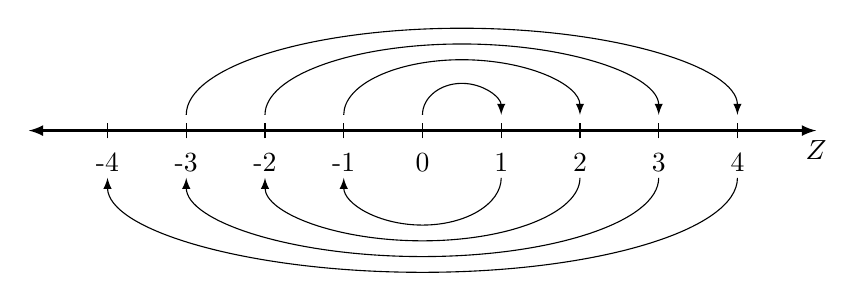
\begin{tikzpicture}[%
        >=latex
    ]
        \draw[<->, thick] (-5, 0) to (5, 0) node[below] {$\mathbb{Z}$};
        \foreach\x in {-4, -3, -2, -1, 0, 1, 2, 3, 4}{%
            \draw (\x, -0.1) to (\x, 0.1);
            \node at (\x, -0.4) {\x};
        }
        \draw[->] (0, 0.2) arc(180:0:0.5 and 0.4);
        \draw[->] (1, -0.6) arc(0:-180:1 and 0.6);
        \draw[->] (-1, 0.2) arc(180:0:1.5 and 0.7);
        \draw[->] (2, -0.6) arc(0:-180:2 and 0.8);
        \draw[->] (-2, 0.2) arc(180:0:2.5 and 0.9);
        \draw[->] (3, -0.6) arc(0:-180:3 and 1);
        \draw[->] (-3, 0.2) arc(180:0:3.5 and 1.1);
        \draw[->] (4, -0.6) arc(0:-180:4 and 1.2);
    \end{tikzpicture}
\end{document}
            \caption{Diagram of a Bijection Between
                     $\mathbb{N}$ and $\mathbb{Z}$.}
            \label{fig:Bijection_N_and_Z}
        \end{figure}
        One of the standard results about countable sets is
        that their subsets are also countable. This theorem
        relies, in a very subtle way, the use of the axiom
        of choice. There are a few stepping stones to get
        there. We will accept the various
        Cantor-Schr\"{o}eder-Bernstein theorems, which say
        the following:
        \begin{ltheorem}
              {First Cantor-Schr\"{o}eder-Bernstein Theorem}
              {First_Cantor_Schroeder_Bernstein}
            If $A$ and $B$ are sets such that there is an injective
            function $f:A\rightarrow{B}$ and an injective function
            $g:B\rightarrow{A}$, then there is a bijective function
            $h:A\rightarrow{B}$.
        \end{ltheorem}
        \begin{ltheorem}
              {Second Cantor-Schr\"{o}eder-Bernstein Theorem}
              {Second_Cantor_Schroeder_Bernstein}
            If $A$ and $B$ are sets such that there is a surjective
            function $f:A\rightarrow{B}$ and a surjective function
            $g:B\rightarrow{A}$, then there is a bijective function
            $h:A\rightarrow{B}$.
        \end{ltheorem}
        \par\hfill\par
        Using cardinalities, this says that if
        $\Card(A)\leq\Card(B)$ and $\Card(B)\leq\Card(A)$, then
        $\Card(A)=\Card(B)$. With this notation it becomes more
        intuitive. We will use this to prove that various sets are
        countable. Many sets that appear to be larger than $\mathbb{N}$
        can shown to to be the same size as $\mathbb{N}$ by finding
        a simple injective function, without finding an explicit
        bijection.
        \begin{ltheorem}
              {Third Cantor-Schr\"{o}eder-Bernstein Theorem}
              {Third_Cantor_Schroeder_Bernstein}
            If $A$, $B$, and $C$ are sets such that
            $A\subseteq{B}\subseteq{C}$, and if $A$ and $C$ are equivalent
            sets, then $B$ and $C$ are equivalent sets.
        \end{ltheorem}
        \par\hfill\par
        This says that if $\Card(A)\leq\Card(B)\leq\Card(C)$,
        and if $\Card(A)=\Card(C)$, then $\Card(B)=\Card(C)$.
        \begin{theorem}
            \label{thm:Measure_Theory_NxN_Is_Countable}
            $\mathbb{N}\times\mathbb{N}$ is countably infinite.
        \end{theorem}
        \begin{proof}
            There is a trivial injection
            $f:\mathbb{N}\rightarrow\mathbb{N}\times\mathbb{N}$
            defined by:
            \begin{equation}
                f(n)=(n,0)
            \end{equation}
            There is also an injection
            $g:\mathbb{N}\times\mathbb{N}\rightarrow\mathbb{N}$
            defined by:
            \begin{equation}
                g(n.m)=2^{n}3^{m}
            \end{equation}
            Since 2 and 3 are co-prime, if
            $g(n_{1},m_{1})=g(n_{2},m_{2})$, then
            $(n_{1},m_{1})=(n_{2},m_{2})$. Thus, $g$ is an injection.
            By the Cantor-Schr\"{o}eder-Bernstein Theorem, there is a
            bijection $h:\mathbb{N}\rightarrow\mathbb{N}\times\mathbb{N}$.
        \end{proof}
        One can intuitively see that the set of all positive
        rational numbers $\mathbb{Q}^{+}$ is countable by examining
        the zig-zag pattern shown in
        Fig.~\ref{fig:Bijection_N_and_Q_Plus}.
        Thm.~\ref{thm:Measure_Theory_NxN_Is_Countable} also
        shows this in a more rigorous way that. We can create
        a one-to-one correspondence with
        $\mathbb{N}\times\mathbb{N}$ by mapping
        $pq^{\minus{1}}\mapsto(p,q)$. Thus $\mathbb{Q}^{+}$
        and $\mathbb{N}\times\mathbb{N}$ are equivalent sets.
        But $\mathbb{N}\times\mathbb{N}$ and $\mathbb{N}$
        are equivalent sets, and therefore $\mathbb{Q}^{+}$
        is countable.
        Thm.~\ref{thm:Measure_Theory_NxN_Is_Countable} can also be used
        to show that the countable union of countable sets is also
        countable.
        \begin{ltheorem}{Equivalence of Countable Sets}
              {Countable_iff_exists_inj_to_N}
            A set $A$ is countable if and only if there is an injective
            function $f:A\rightarrow\mathbb{N}$.
        \end{ltheorem}
        Thm.~\ref{thm:Countable_iff_exists_inj_to_N} seems
        intuitively obvious, the injective function is
        simply the listing function. For a finite set, this
        is precisely how one constructs such an injection.
        For an infinite set $A$, this is equivalent to
        showing that any infinite subset of $\mathbb{N}$ is
        equivalent to $\mathbb{N}$. The standard proof
        using \textit{induction}, but actually has the axiom
        of choice underlying it.
        \begin{theorem}
            If $\mathcal{A}$ is a countably infinite set
            such that, for all $A\in\mathcal{A}$, $A$ is
            a non-empty countable set, then the set:
            \begin{equation}
                S=\bigcup_{A\in\mathcal{A}}A
            \end{equation}
            Is a countable set.
        \end{theorem}
        \begin{proof}
            If $\mathcal{F}$ is finite, then we are done. Suppose not.
            Let $A:\mathbb{N}\rightarrow\mathcal{A}$ be a bijection,
            and define:
            \begin{equation}
                S=\bigcup_{n\in\mathbb{N}}A_{n}
            \end{equation}
            Also, let:
            \begin{equation}
                \mathcal{F}_{n}
                =\{f:A_{n}\rightarrow\mathbb{N}:
                    f\textrm{ is injective}\}
            \end{equation}
            Since, for all $n\in\mathbb{N}$, $A_{n}$ is
            non-empty and countable, $\mathcal{F}_{n}$
            is non-empty. Let:
            \begin{equation}
                \mathcal{F}
                =\bigcup_{n\in\mathbb{N}}\mathcal{F}_{n}
            \end{equation}
            Thus, by the axiom of choice, there is a function
            $F:\mathbb{N}\rightarrow\mathcal{F}$ such that, for all
            $n\in\mathbb{N}$, $F_{n}\in\mathcal{F}_{n}$. For
            $x\in{S}$, let:
            \begin{equation}
                \varphi_{x}
                =\inf\{n\in\mathbb{N}:x\in{A}_{n}\}
            \end{equation}
            By the well-ordering of $\mathbb{N}$, for all
            $x\in{S}$, $\varphi_{x}$ is well defined. Let
            $\phi:S\rightarrow\mathbb{N}\times\mathbb{N}$
            be defined by:
            \begin{equation}
                \phi(x)
                =\big(\varphi_{x},F_{\varphi_{x}}(x)\big)
            \end{equation}
            Then $\phi$ is an injection. For if
            $\big(\varphi_{x},F_{\varphi_{x}}(x)\big)=%
             \big(\varphi_{y},F_{\varphi_{x}}(y)\big)$, then
            $\varphi_{x}=\varphi_{y}$, and thus
            $F_{\varphi(x)}(x)=F_{\varphi(x)}(y)$. But
            $F_{\varphi_{x}}$ is an injection, and
            thus $x=y$. Therefore $\phi$ is an injection.
            But $\mathbb{N}\times\mathbb{N}$ and $\mathbb{N}$
            are equivalent sets, and thus there's an
            injection $f:\mathbb{N}\times\mathbb{N}$. And
            the composition of injective functions is again
            injective, and thus
            $\phi\circ{f}:S\rightarrow\mathbb{N}$ is an
            injective function. But by
            Thm.~\ref{thm:Countable_iff_exists_inj_to_N},
            if there is an injective function
            $f:S\rightarrow\mathbb{N}$, then $S$ is
            countable. Therefore, etc.
        \end{proof}
        \begin{theorem}
            If $X$ is infinite, then there exists a
            countably infinite set $A\subseteq{X}$.
        \end{theorem}
        \begin{proof}
            If $A$ is finite, then we are done. Suppose not.
            For $n\in\mathbb{N}$, let:
            \begin{equation}
                A_{n}
                =\{g:\mathbb{Z}_{n}\rightarrow{A}:f\textrm{ is inective}\}
            \end{equation}
            Also, define:
            \begin{equation}
                \mathcal{F}=\bigcup_{n\in\mathbb{N}}A_{n}
            \end{equation}
            But by the axiom of choice, there is a function
            $f:\mathbb{N}\rightarrow\mathcal{F}$ such that
            $f_{n}\in{A}_{n}$. But then, for all
            $n\in\mathbb{N}$, the range of $f_{n}$ is finite.
            \begin{equation}
                A=\bigcup_{n\in\mathbb{N}}f_{n}
                    \Big(\mathbb{Z}_{n}\Big)
            \end{equation}
            Then $A\subseteq{X}$ is countably infinite.
        \end{proof}
        The set of rational numbers, $\mathbb{Q}$, is also
        countable. We may intuitively think of $\mathbb{N}$
        as being smaller than $\mathbb{Q}$, since there are
        simple \textit{surjections} that can be constructed
        from $\mathbb{Q}$ to $\mathbb{N}$. There is also a
        surjection from $\mathbb{N}$ onto $\mathbb{Q}^{+}$,
        as is shown in Fig.~\ref{fig:Bijection_N_and_Q_Plus}.
        To construct such a surjection, write out all of the
        positive rational numbers in a grid so that $a_{nm}$
        is the number $n/m$. Then zig-zag along the diagonals
        to construct the function. Thus there is a surjection
        $f:\mathbb{Q}^{+}\rightarrow\mathbb{N}$ and a surjection
        $g:\mathbb{N}\rightarrow\mathbb{Q}^{+}$. The
        Cantor-Schr\"{o}eder-Bernstein theorem says that if there is
        surjection from $A$ to $B$ and a surjection from $B$ to $A$, then
        there is a bijection between $A$ and $B$. Therefore there is a
        bijection between $\mathbb{N}$ and $\mathbb{Q}^{+}$, and
        $\mathbb{Q}^{+}$ is countable.
        \begin{figure}[H]
            \centering
            \captionsetup{type=figure}
            \resizebox{0.7\textwidth}{!}{%
                \documentclass[crop,class=article]{standalone}
%----------------------------Preamble-------------------------------%
\usepackage{tikz}
\usetikzlibrary{arrows.meta}
%--------------------------Main Document----------------------------%
\begin{document}
    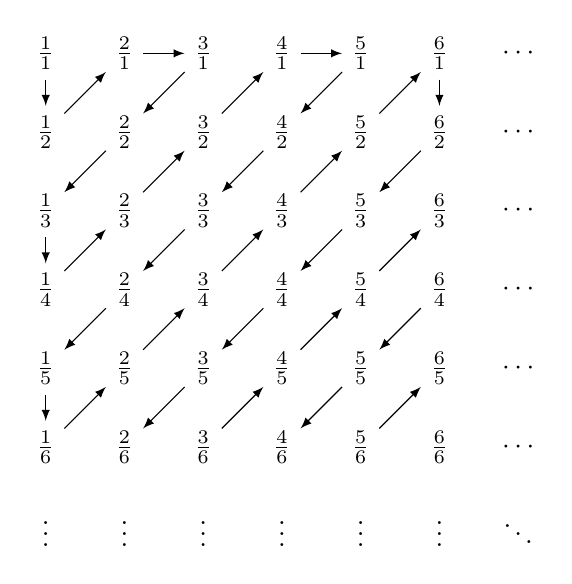
\begin{tikzpicture}[%
        >=latex
    ]
        \foreach\y in {1, 2, 3, 4, 5, 6}{%
            \foreach\x in {1, 2, 3, 4, 5, 6}{%
                \node (\x\y) at (\x, 7-\y) {$\frac{\x}{\y}$};
            }
        }
        \foreach\x in {1, 2, 3, 4, 5, 6}{%
            \node at (7, \x) {$\cdots$};
            \node at (\x, 0) {$\vdots$};
        }
        \node at (7, 0) {$\ddots$};
        \draw[->] (11) to (12);
        \draw[->] (12) to (21);
        \draw[->] (21) to (31);
        \draw[->] (31) to (22);
        \draw[->] (22) to (13);
        \draw[->] (13) to (14);
        \draw[->] (14) to (23);
        \draw[->] (23) to (32);
        \draw[->] (32) to (41);
        \draw[->] (41) to (51);
        \draw[->] (51) to (42);
        \draw[->] (42) to (33);
        \draw[->] (33) to (24);
        \draw[->] (24) to (15);
        \draw[->] (15) to (16);
        \draw[->] (16) to (25);
        \draw[->] (25) to (34);
        \draw[->] (34) to (43);
        \draw[->] (43) to (52);
        \draw[->] (52) to (61);
        \draw[->] (61) to (62);
        \draw[->] (62) to (53);
        \draw[->] (53) to (44);
        \draw[->] (44) to (35);
        \draw[->] (35) to (26);
        \draw[->] (36) to (45);
        \draw[->] (45) to (54);
        \draw[->] (54) to (63);
        \draw[->] (64) to (55);
        \draw[->] (55) to (46);
        \draw[->] (56) to (65);
    \end{tikzpicture}
\end{document}
            }
            \caption{Diagram of a Surjection from
                     $\mathbb{N}$ onto $\mathbb{Q}^{+}$.}
            \label{fig:Bijection_N_and_Q_Plus}
        \end{figure}
        We can modify Fig.~\ref{fig:Bijection_N_and_Q_Plus}
        slightly to create a surjection between $\mathbb{N}$
        and $\mathbb{Q}$, see
        Fig.~\ref{fig:Bijection_N_and_Q}.
        It is important to note that this bijection will not
        preserve the order of the rational numbers. The
        bijection will have to jump around back and forth.
        Any such bijection will be forced to do this, as the
        rationals are everywhere dense on $\mathbb{R}$. Any
        monotonic sequence of $\mathbb{Q}$ cannot possibly
        be a bijection.
        \begin{theorem}
            If $A$ is a countably infinite set and
            $B\subseteq{A}$, then $B$ is countable.
        \end{theorem}
        \begin{proof}
            As $A$ is countably infinite, there is a bijection
            $a:\mathbb{N}\rightarrow{A}$. Define:
            \begin{equation}
                K=\{n\in\mathbb{N}:a_{n}\in{B}\}
            \end{equation}
            As $B\subseteq{A}$,
            this set contains a subsequence of points in
            $\mathbb{N}$ that get mapped into $B$. If $K$ is finite,
            then $B$ is finite, and if not then $K$ is countably
            infinite, and thus $B$ is countably infinite.
        \end{proof}
        \begin{figure}[H]
            \centering
            \captionsetup{type=figure}
            \resizebox{\textwidth}{!}{%
                \documentclass[crop,class=article]{standalone}
%----------------------------Preamble-------------------------------%
\usepackage{tikz}
\usepackage{amsmath}
\usetikzlibrary{arrows.meta}
%--------------------------Main Document----------------------------%
\begin{document}
    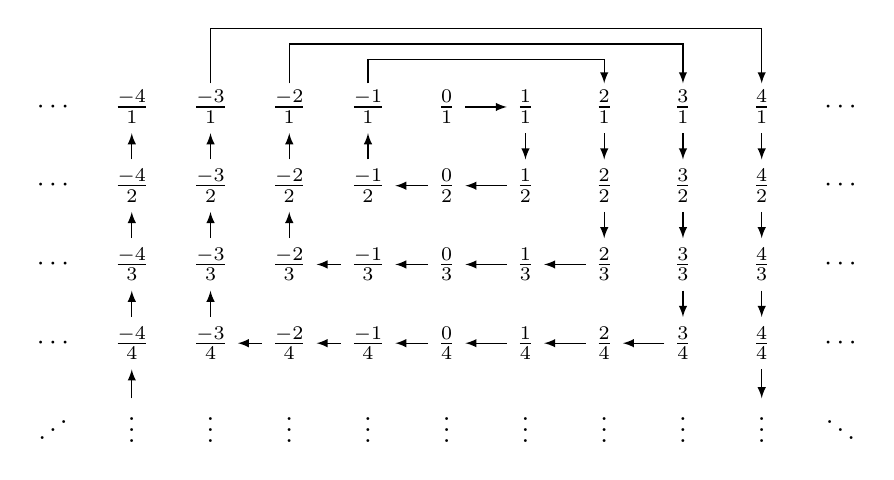
\begin{tikzpicture}[%
        >=latex
    ]
        \foreach\y in {1, 2, 3, 4}{%
            \foreach\x in {-4, -3, -2, -1, 0, 1, 2, 3, 4}{%
                \node (\x\y) at (\x, 7-\y) {$\frac{\x}{\y}$};
            }
        }
        \foreach\x in {-4, -3, -2, -1, 0, 1, 2, 3, 4}{%
            \node at (\x, 2) {$\vdots$};
        }
        \foreach\y in {3, 4, 5, 6}{%
            \node at (5, \y) {$\cdots$};
            \node at (-5, \y) {$\cdots$};
        }
        \node at (5, 2) {$\ddots$};
        \node at (-5, 2) {$\reflectbox{\ensuremath{\ddots}}$};
        \draw[->] (01) to (11);
        \draw[->] (11) to (12);
        \draw[->] (12) to (02);
        \draw[->] (02) to (-12);
        \draw[->] (-12) to (-11);
        \draw[->] (-1, 6.3) to (-1, 6.6)
                            to (2, 6.6)
                            to (2, 6.3);
        \draw[->] (21) to (22);
        \draw[->] (22) to (23);
        \draw[->] (23) to (13);
        \draw[->] (13) to (03);
        \draw[->] (03) to (-13);
        \draw[->] (-13) to (-23);
        \draw[->] (-23) to (-22);
        \draw[->] (-22) to (-21);
        \draw[->] (-2, 6.3) to (-2, 6.8)
                            to (3, 6.8)
                            to (3, 6.3);
        \draw[->] (31) to (32);
        \draw[->] (32) to (33);
        \draw[->] (33) to (34);
        \draw[->] (34) to (24);
        \draw[->] (24) to (14);
        \draw[->] (14) to (04);
        \draw[->] (04) to (-14);
        \draw[->] (-14) to (-24);
        \draw[->] (-24) to (-34);
        \draw[->] (-34) to (-33);
        \draw[->] (-33) to (-32);
        \draw[->] (-32) to (-31);
        \draw[->] (-3, 6.3) to (-3, 7)
                            to (4, 7)
                            to (4, 6.3);
        \draw[->] (41) to (42);
        \draw[->] (42) to (43);
        \draw[->] (43) to (44);
        \draw[->] (44) to (4, 2.3);
        \draw[->] (-4, 2.3) to (-44);
        \draw[->] (-44) to (-43);
        \draw[->] (-43) to (-42);
        \draw[->] (-42) to (-41);
    \end{tikzpicture}
\end{document}
            }
            \caption{Diagram of a Surjection from
                     $\mathbb{N}$ onto $\mathbb{Q}$.}
            \label{fig:Bijection_N_and_Q}
        \end{figure}
        \begin{theorem}
            If $A$ is an infinite set, then there exists a
            countable subset $B\subseteq{A}$.
        \end{theorem}
        \begin{proof}
            If $A$ is infinite then there is an
            $a_{1}\in{A}$. But, as $A$ is infinite,
            $A\setminus\{a_{1}\}$ is infinite, and there
            is an $a_{2}\in{A}\setminus\{a_{1}\}$. Continuing
            we obtain a sequence of distinct elements in $A$.
            Let $B=\{a_{n}:n\in\mathbb{N}\}$. Then
            $B\subseteq{A}$, and $B$ is countable.
        \end{proof}
        \begin{lexample}
            Suppose we have a collection of disjoint intervals
            of $\mathbb{R}$. This collection is either finite
            or countable. For in every interval, choose a
            rational number $q_{n}$. Let
            $A=\{q_{1},q_{2},\hdots\}$. Then
            $A\subseteq\mathbb{Q}$, and thus $A$ is either
            finite or countable. But this is also an enumeration
            of the intervals in the collection, and thus the
            collection is either finite or countable.
        \end{lexample}
        Given a countable collection of sets
        $A=\{\mathcal{A}_{1},\mathcal{A}_{2},\hdots\}$ such
        that, for all $n\in\mathbb{N}$, $\mathcal{A}_{n}$ is
        also a countable set, then the union is countable. That is:
        \begin{equation}
            B=\bigcup_{n=1}^{\infty}\mathcal{A}_{n}
        \end{equation}
        is a countable set. The proof of this is a mimicry of
        the proof of the countability of $\mathbb{Q}$. Not
        every set is either finite or countable. The real numbers,
        $\mathbb{R}$, is an example of an \textit{uncountable}
        set. First, some notes on the power set of a set.
        \begin{ldefinition}{Power Set}
            The power set of a set $\Omega$, denoted
            $\mathcal{P}(\Omega)$, is the set of all subsets of
            $\Omega$:
            \begin{equation}
                \mathcal{P}(\Omega)=
                \{A:A\subseteq\Omega\}
            \end{equation}
        \end{ldefinition}
        \begin{lexample}{}{}
            \begin{subequations}
                If $\Omega=\{1,2\}$, then the power set is:
                \begin{equation}
                    \mathcal{P}(\Omega)=
                    \big\{\emptyset,\{1\},\{2\},\{1,2\}\big\}
                \end{equation}
                We must consider the empty set, since for any set
                $A$, $\emptyset\subseteq{A}$. As another example,
                let $\Omega=\{1,2,3\}$. Then:
                \begin{equation}
                    \mathcal{P}(\Omega)=
                    \big\{\emptyset,\{1\},\{2\},\{3\},\{1,2\},
                      \{1,3\},\{2,3\},\{1,2,3\}\big\}
                \end{equation}
                We see that, in the first example, a set with
                2 elements has a power set with 4 elements. In the
                second example we see that a set with 3 elements has
                a power set with 8 elements. This pattern continues
                for finite sets. If $A$ has $n$ elements, then
                $\mathcal{P}(A)$ has $2^{n}$ elements. If
                $A$ is an infinite set, then $\mathcal{P}(A)$ is
                uncountable. Indeed:
                \begin{equation}
                    \Card\big(\mathcal{P}(\mathbb{N})\big)=
                    \Card(\mathbb{R})
                \end{equation}
                We can show this by using the binary representation
                of real numbers. We construct a bijection as
                follows: If $A\subseteq\mathbb{N}$, then
                let $r_{A}=0.n_{1}n_{2}\hdots$ where:
                \begin{equation}
                    n_{i}=
                    \begin{cases}
                        0,&i\notin{A}\\
                        1,&i\in{A}
                    \end{cases}
                \end{equation}
                The function
                $f:\mathcal{P}(\mathbb{N})\rightarrow[0,1]$
                defined by $f(A)=r_{A}$ is thus a bijection.
                That is, every element of $[0,1]$ gets mapped to in
                a one-to-one manner. The potentially tricky numbers are
                0 and 1, but $f(\emptyset)=0$, and $f(\mathbb{N})=1$.
                Thus $\mathcal{P}(\mathbb{N})$ and $[0,1]$ are of the
                same cardinality. But $(0,1)$ and $\mathbb{R}$
                are of the same cardinality. To see this, consider
                the graph of the function
                $g:(0,1)\rightarrow\mathbb{R}$ defined as:
                \begin{equation}
                    g(x)=\frac{2x-1}{x(1-x)}
                \end{equation}
                This is a bijection between the unit interval
                $(0,1)$ and $\mathbb{R}$. One can also use the
                \textit{stereographic projection} to show this.
                But also $[0,1]$ and $(0,1)$ have the same cardinality.
                For this, consider the following function:
                \begin{equation}
                    f(x)=
                    \begin{cases}
                        \frac{1}{2},&x=0\\
                        \frac{1}{2^{n+2}},&x=\frac{1}{2^{n}}\\
                        x,&\textrm{Otherwise}
                    \end{cases}
                \end{equation}
                A graph of this is shown in
                Fig.~\ref{fig:Measure_Theory_Bijection_Closed_I_to_Open}.
                Therefore, $\mathbb{R}$ and
                $\mathcal{P}(\mathbb{N})$ have the same cardinality.
                This can then be used to show that $\mathbb{R}$ is
                uncountable.
            \end{subequations}
        \end{lexample}
        \begin{figure}[H]
            \centering
            \captionsetup{type=figure}
            \documentclass[crop,class=article]{standalone}
%----------------------------Preamble-------------------------------%
\usepackage{tikz}                       % Drawing/graphing tools.
\usetikzlibrary{arrows.meta}            % Latex and Stealth arrows.
%--------------------------Main Document----------------------------%
\begin{document}
    \begin{tikzpicture}[>=Latex, scale=2]
        \draw[->] (-0.15in, 0) to (1.1in, 0) node[above] {$x$};
        \draw[->] (0, -0.15in) to (0, 1.1in) node[right] {$y$};
        \draw (0, 0) to (1in, 1in);
        \draw[fill=black, draw=black] (0, 0.5in) circle (0.3mm);
        \foreach\x in{1in, 0.5in, 0.25in, 0.125in, 0.0625in, 0.03125in}{
            \draw[fill=white, draw=black] (\x, \x) circle (0.3mm);
            \draw[fill=black, draw=black] (\x, 0.25*\x) circle (0.3mm);
        }
    \end{tikzpicture}
\end{document}
            \caption{Bijection from $[0,1]$ to $(0,1)$.}
            \label{fig:Measure_Theory_Bijection_Closed_I_to_Open}
        \end{figure}
        The power set of any set is strictly larger than the
        original set. If $\Omega$ is finite with $n$ elements, it
        can be shown that $\mathcal{P}(\Omega)$ has $2^{n}$
        eleents. For infinite sets, there is a trivial surjection
        from $\mathcal{P}(\Omega)$ onto $\Omega$: for any element
        $x$, let $f(\{x\})=x$. This shows that
        $\Card(\Omega)\leq\Card(\mathcal{P}(\Omega))$. We now show
        that the inequality is strict.
        \begin{theorem}
            If $\Omega$ is a set, then there is no bijection
            $f:\Omega\rightarrow\mathcal{P}(\Omega)$
        \end{theorem}
        \begin{proof}
            For suppose not, and let
            $f:\Omega\rightarrow\mathcal{P}(\Omega)$ be such a
            bijection. Define:
            \begin{equation}
                A=\{x\in\Omega:x\in{f}(x)\}
            \end{equation}
            Then $A\subseteq\Omega$, and thus
            $A\in\mathcal{P}(\Omega)$. But then the complement of
            $A$ is also an element of $\mathcal{P}(\Omega)$. But
            $f$ is a bijection and thus there is an $x\in\Omega$
            such that $f(x)=A^{C}$. If $x\in{f}(x)$, then
            $x\in{A}$, a contradiction as $f(x)=A^{C}$, and thus
            $x\in{A}^{C}$ as well. Therefore $x\notin{f}(x)$. But
            then $x\in{A}^{C}$. But, from the definition of $A$,
            since $x\in{A}^{C}$ and $f(x)=A^{C}$, $x\in{f}(x)$
            and thus $x\in{A}$, a contradiction. Thus there is no
            $x$ such that $f(x)=A^{C}$. Therefore, $f$ is not a
            bijection.
        \end{proof}
        From this we conclude that $\mathcal{P}(\mathbb{N})$
        is an uncountable infinite set. But since $\mathbb{R}$
        and $\mathcal{P}(\mathbb{N})$ have the same cardinality,
        $\mathbb{R}$ is also uncountable.
        If a set $A$ has the same cardinality as $\mathbb{R}$,
        we say that $A$ has the cardinality of the continuum.
        \begin{lexample}
            There is a bijection between the open unit
            square $(0,1)\times(0,1)$ and the open unit interval
            $(0,1)$. For an element $(x,y)\in(0,1)\times(0,1)$,
            let $z\in(0,1)$ be defined as
            $z=0.x_{1}y_{1}x_{2}y_{2}x_{3}y_{3}\dots$ This is
            a bijection, for all $(x,y)$ in the square there is
            a corresponding $z\in(0,1)$, and for all
            $z\in(0,1)$ there is a corresponding element of
            $(0,1)\times(0,1)$. We can say that $(x,y)$ can
            be coded into $z$, and $z$ can be decoded into
            $(x,y)$. Hence, $(0,1)\times(0,1)$ has the cardinality
            of the continuum. By stereographic projection and induction
            we obtain:
            \par\hfill\par
            \begin{subequations}
                \begin{minipage}[b]{0.49\textwidth}
                    \begin{equation}
                        \Card(\mathbb{R}^{2})=\Card(\mathbb{R})
                    \end{equation}
                \end{minipage}
                \hfill
                \begin{minipage}[b]{0.49\textwidth}
                    \begin{equation}
                        \Card(\mathbb{R}^{n})=\Card(\mathbb{R})
                    \end{equation}
                \end{minipage}
                \par
            \end{subequations}
        \end{lexample}
        \begin{lexample}
            Consider the set of all real-valued sequences. We've seen
            that any real number can be represented as a function
            $f:\mathbb{N}\rightarrow\{0,1\}$. A real-valued sequence
            is a function $a:\mathbb{N}\rightarrow\mathbb{R}$, and
            thus the set of real-valued sequences can be seen as the
            set of functions whose domain is $\mathbb{N}$ and whose
            range is the set of all functions
            $f:\mathbb{N}\rightarrow\{0,1\}$. So given a sequence
            $a$, the image of $a_{n}$, for $n\in\mathbb{N}$, is a
            function $f_{n}:\mathbb{N}\rightarrow\{0,1\}$. Therefore
            the set of all real-valued sequences can be represented
            as the set of all functions
            $g:\mathbb{N}\times\mathbb{N}\rightarrow\{0,1\}$, where
            $g(n,m)=f_{n}(m)$. But $\mathbb{N}\times\mathbb{N}$ is
            countable, and thus the set of all functions of the form
            $g:\mathbb{N}\times\mathbb{N}\rightarrow\{0,1\}$ has the
            same cardinality as the set of all functions of the form
            $f:\mathbb{N}\rightarrow\{0,1\}$. But this has the
            cardinality of the continuum. Therefore, the set of all
            real-valued sequences has the cardinality of the continuum.
        \end{lexample}
\section{Basic Concepts}
    \subsection{Sets}
        \subsubsection{Cartesian Products}
            \begin{lexample}{}{}
                One example of a Cartesian product
                is the Euclidean plane, $\mathbb{R}^{2}$. This is
                the set:
                \begin{equation}
                    \mathbb{R}^{2}=\mathbb{R}\times\mathbb{R}
                \end{equation}
                Where $\mathbb{R}$ denotes the set of real numbers.
                $\mathbb{R}^{2}$ is thus the set of all ordered
                pairs of real numbers. This is the same thing as
                the \textit{Cartesian} plane. Points
                in the Cartesian plane are identified by their
                \textit{coordinates}, $P=(x,y)$.
            \end{lexample}
            \begin{lexample}{}{Cartesian_Product}
                For the sake of computation, consider the
                set $A=\{1,2,3\}$ and $B=\{a,b\}$. We can then
                compute $A\times{B}$ directly:
                \begin{equation}
                    A\times{B}=\big\{(1,a),(1,b),(2,a),(2,b),
                        (3,a),(3,b)\big\}
                \end{equation}
                We can also compute $A\times{A}$ and $B\times{B}$:
                \begin{subequations}
                    \begin{align}
                        A\times{A}&=\big\{
                            (1,1),(1,2),(1,3),
                            (2,1),(2,2),(2,3),
                            (3,1),(3,2),(3,3)\big\}\\
                        B\times{B}&=\big\{
                            (a,a),(a,b),(b,a),(b,b)\big\}
                    \end{align}
                \end{subequations}
                Lastly, compute $B\times{A}$:
                \begin{equation}
                    B\times{A}=\big\{
                        (a,1),(a,2),(a,3),
                        (b,1),(b,2),(b,3)\big\}
                \end{equation}
                Note that, since for distinct elements $\alpha$
                and $\beta$, we have that
                $(\alpha,\beta)\ne(\beta,\alpha)$, and thus
                the Cartesian products $A\times{B}$ and $B\times{A}$
                are not equal, in general. Equality is obtained
                if and only if $A=B$.
            \end{lexample}
            Note that in Ex.~\ref{ex:Cartesian_Product}, the
            \textit{size} of the Cartesian product of two sets
            was simply the product of the number of elements of
            the constituent sets. That is, we see that $A$ has
            three elements and $B$ has two elements, but also
            that $A\times{B}$ has six elements. Moreover,
            $A\times{A}$ has nine elements, and $B\times{B}$ has
            four. This pattern holds for \textit{finite} sets.
            To be precise, we need to define what finite sets
            are, and what are \textit{infinite} sets. To do
            this we need the notion of a function.
    \subsection{Cardinality}
        We begin by talking about cardinality. This is the
        \textit{size} of a set. For an infinite set it
        doesn't make sense to talk about the \textit{number}
        of elements, but we can specify what it means two sets
        to have the same size. Sets $A$ and $B$ are equivalent
        if there exists a bijection $f:A\rightarrow{B}$.
        We then say that $A$ and $B$ have the same cardinality.
        The notation is written as $|A|=|B|$ or
        $\Card(A)=\Card(B)$. A finite set is a set $A$ such that
        there is a bijection between $A$ and $\mathbb{Z}_{n}$.
        We can then view the elements of $A$ as
        $A=\{a_{1},\hdots,a_{n}\}$. A countable set is a set
        $A$ such that there is a bijection between $A$ and
        $\mathbb{N}$. Here, $\mathbb{N}$ is the set of all
        natural numbers, or positive integers.
    \subsection{Set Operations}
        There are several operations that can be performed on sets,
        most notable are union, intersection, difference, and symmetric
        difference.
        These two concepts can be visualized with Venn diagrams, as shown in
        Fig.~\ref{fig:MEASURE_THEORY_union_intersection_venn_diagram}.
        If $A$ and $B$ are sets, and if $C\subseteq{A}\cup{B}$, then
        either $C\subseteq{A}$ or $C\subseteq{B}$, or both. It is
        possible that $C\subseteq{A}\cup{B}$ and yet $C$ and $B$ have no
        elements in common, as long as $C\subseteq{A}$. As an example,
        take $A$ and $B$ to be disjoint sets. Then $A\subseteq{A}\cup{B}$,
        yet $A$ and $B$ have no elements in common. If
        $C\subseteq{A}\cap{B}$, then it must be true that
        $C\subseteq{A}$ and $C\subseteq{B}$.
        As with the notions of unions and intersections, set differences and
        symmetric differences can be visualized using Venn diagrams.
        \begin{theorem}
            \label{thm:MEASURE_THEORY_SET_DIFFERENCE_AS_INTERSECTION}
            If $A$, $B$, and $C$ are sets, and if $A\subseteq{C}$
            and $B\subseteq{C}$, then:
            \begin{equation}
                B\setminus{A}=B\cap(C\setminus{A})
            \end{equation}
        \end{theorem}
        \begin{proof}
            For if $x\in{B}\setminus{A}$, then
            $x\in{B}$ and $x\notin{A}$. But
            $B\subseteq{C}$, and thus if $x\in{B}$, then $x\in{C}$.
            But if $x\notin{A}$, then $x\in{C}\setminus{A}$. Therefore
            $B\setminus{A}\subseteq{B}\cap(C\setminus{A})$.
            Similarly, $B\cap(C\setminus{A})\subseteq{B}\setminus{A}$,
            and therefore $B\setminus{A}={B}\cap(C\setminus{A})$.
        \end{proof}
        While set difference appears similar to subtraction that one finds in
        basic arithmetic, the two have their differences. For any two real
        numbers $a$ and $b$, $b=a-(a-b)$. For sets this is not true. For let
        $A$ be the empty set, and let $B$ be non-empty. Then
        $A\setminus(A\setminus{B})=\emptyset$, which is not $B$.
        Also, while it may seems convincing that
        $A\setminus(B\setminus{A})=A\setminus{B}$, this is not true. For
        let $A$ be a non-empty set and let $B=A$. Then
        $A\setminus(B\setminus{A})=A$, but $A\setminus{B}=\emptyset$.
        The concept of set difference can then be used to define the
        concept of complement.
        \begin{ldefinition}{Complement}
            The complement of a set $A$ with respect to a set
            $\Omega$, denoted $A^{C}$, is the set:
            \begin{equation}
                A^{C}=\Omega\setminus{A}
            \end{equation}
        \end{ldefinition}
        Thm.~\ref{thm:MEASURE_THEORY_SET_DIFFERENCE_AS_INTERSECTION} can then
        be translated into the notation of complements as follows:
        With this, we can prove some results about set differences.
        \begin{theorem}
            If $A$ and $B$ are sets, then:
            \begin{equation}
                A=\big(A\cap{B}\big)\cup\big(A\setminus{B}\big)
            \end{equation}
        \end{theorem}
        \begin{proof}
            For:
            \begin{subequations}
                \begin{align}
                    \big(A\cap{B})\cup\big(A\setminus{B}\big)
                    &=\big(A\cap{B}\big)\cup\big(A\cap{B}^{C}\big)\\
                    &=A\cap(B\cup{B}^{C})\\
                    &=A\cap\Omega\\
                    &=A
                \end{align}
            \end{subequations}
        \end{proof}
        \begin{theorem}
            If $A$, $B$, and $C$ are sets, then:
            \begin{equation}
                A\cap\big(B\setminus{C}\big)
                =\big(A\cap{B}\big)\cap\big(A\setminus{C}\big)
            \end{equation}
        \end{theorem}
        \begin{proof}
            For:
            \begin{subequations}
                \begin{align}
                    A\cap\big(B\setminus{C}\big)
                    &=A\cap\big(B\cap{C}^{C}\big)\\
                    &=\big(A\cap{A}\big)\cap\big(B\cap{C}^{C}\big)\\
                    &=\big(A\cap{B}\big)\cap\big(A\cap{C}^{C}\big)\\
                    &=\big(A\cap{B}\big)\cap\big(A\setminus{C}\big)
                \end{align}
            \end{subequations}
        \end{proof}
        Intersections do distribute over set differences.
        \begin{theorem}
            If $A$, $B$, and $C$ are sets, then:
            \begin{equation}
                A\cap(B\setminus{C})=
                (A\cap{B})\setminus(A\cap{C})
            \end{equation}
        \end{theorem}
        \begin{proof}
            For:
            \begin{subequations}
                \begin{align}
                    \big(A\cap{B}\big)\setminus\big(A\cap{C}\big)
                    &=\big(A\cap{B}\big)\cap\big(A\cap{C}\big)^{C}\\
                    &=\big(A\cap{B}\big)\cap\big(A^{C}\cup{C}^{C}\big)\\
                    &=\Big(\big(A\cap{B}\big)\cap{A}^{C}\Big)
                        \cup\Big(\big({A}\cap{B}\big)\cap{C}^{C}\Big)\\
                    &=\Big(\big(A\cap{A}^{C}\big)\cap{B}\Big)\cup
                        \Big(\big(A\cap{B}\big)\cap{C}^{C}\Big)\\
                    &=\emptyset\cup
                        \Big(\big(A\cap{B}\big)\cap{C}^{C}\Big)\\
                    &=\big(A\cap{B}\big)\cap{C}^{C}\\
                    &=A\cap\big(B\cap{C}^{C}\big)\\
                    &=A\cap\big(B\setminus{C}\big)
                \end{align}
            \end{subequations}
        \end{proof}
        Unions do not, however. For let $A$ be non-empty and let
        $A=B=C$. Then $A\cup(B\setminus{C})=A$, but
        $(A\cup{B})\setminus(A\cup{C})=\emptyset$.
        \begin{enumerate}
            \item DeMorgan's Laws:
                  \subitem $(A\cup{B})^{C}=A^{C}\cap{B}^{C}$
                  \subitem $(A\cap{B})^{C}=A^{C}\cup{B}^{C}$
        \end{enumerate}
        DeMorgan's Laws hold for arbitrary collections
        of set. If $I$ is some indexing set:
        \begin{align}
            \Big(\bigcup_{\alpha\in{I}}A_{\alpha}\Big)^{C}
            &=\bigcap_{\alpha\in{I}}A_{\alpha}^{C}\\
            \Big(\bigcap_{\alpha\in{I}}A_{\alpha}\Big)^{C}
            &=\bigcup_{\alpha\in{I}}A_{\alpha}^{C}
        \end{align}
        The set operations thus define binary operations
        on the power set of a set $\Omega$. It's important
        to note the notation. An element of $\Omega$ may
        be anything, while an element of
        $\mathcal{P}(\Omega)$ is a subset of $\Omega$.
        That is, the \textit{points} of $\mathcal{P}(\Omega)$
        are themselves sets. Thus, union, intersection,
        etc., define binary operations on
        $\mathcal{P}(\Omega)$. Given two subsets of
        $\Omega$, $A$ and $B$, $A\cup{B}$ is another
        subset of $\Omega$, as is $A\cap{B}$, and so on.
        The complement can also be seen as a unary operator
        on $\mathcal{P}(\Omega)$. From the various theorems
        presented, we have the following:
        \begin{enumerate}
            \item Union is commutative and associative.
            \item Intersection is commutative and
                  associative.
            \item Union distributes over intersection.
            \item Intersection distributes over union.
            \item DeMorgan's Laws hold.
            \item Set difference is not commutative,
                  nor is it associative.
        \end{enumerate}
    \subsection{Sets, Functions, and Countability}
        From set theory, a function $f$ from a set $X$ to a
        set $Y$ is a subset of $X\times{Y}$ such that, for
        all $x\in{X}$, there is a unique $y\in{Y}$
        such that $(x,y)\in{f}$. We often call $X$ the
        domain, $Y$ the range or co-domain, and write
        $f:X\rightarrow{Y}$ to indicate this. The
        \textit{image} of $x\in{X}$ is often written
        as $y=f(x)$. Requiring that $y$ be unique for each
        $x$ is equivalent to the \textit{vertical line test}
        one might find in a calculus course.
        An injective function is a function such
        that $f(x_{1})=f(x_{2})$ if and only if $x_{1}=x_{2}$.
        A surjective function is a function $f:X\rightarrow{Y}$
        such that $f(X)=Y$. That is, every point $y\in{Y}$
        gets mapped to by at least one point in $X$. Or, in
        more familiar notation, for all $y\in{Y}$ there is
        and $x\in{X}$ such that $y=f(x)$. A bijective
        function is a function that is both injective and
        surjective. Sets $X$ and $Y$ such that there
        exists a bijective function $f:X\rightarrow{Y}$ are
        called \textit{equivalent}. Such sets can be said
        to have the same size. We say that $X$ is strictly
        smaller than $Y$ if there is an injective function
        $f:X\rightarrow{Y}$, but no bijective function.
        \begin{definition}
            A finite set is a set $X$ such that there
            exists an $n\in\mathbb{N}$ such that there is
            a bijective function
            $f:\mathbb{Z}_{n}\rightarrow{S}$
        \end{definition}
        \begin{definition}
            A countable set is a set
            $X$ such that there exists a bijective
            function $f:\mathbb{N}\rightarrow{X}$.
        \end{definition}
        Being countable means you can write
        the elements out in a list, or a
        one-to-one correspondence with all of
        the positive integers. Many sets are countable,
        including the whole numbers, integers, rational
        numbers, and \textit{algebraic} numbers. The
        union of finitely many countable sets is also
        countable, as is the union of countably many
        countable sets.
        \begin{example}
            The set of all positive even integers is
            countable. For let $\mathbb{N}_{e}$ be the
            set of all even integers and define
            $f:\mathbb{N}\rightarrow\mathbb{N}_{e}$ be
            $f(n)=2n$ for all $n\in\mathbb{N}$. This is
            a bijection, and thus $\mathbb{N}_{e}$ is
            countable. The set of all odd positive integers
            is countable, as shown by letting
            $f(n)=2n-1$. Even though the set of even
            integers may seem ``smaller,'' than the set of
            all integers, they are equivalent. The set of
            all integers $\mathbb{Z}$ is also countable.
            For let $f:\mathbb{N}\rightarrow\mathbb{Z}$
            be defined as:
            \begin{equation}
                f(n)=
                \begin{cases}
                    \frac{1}{2}(n-1),&n\textrm{ odd}\\
                    -\frac{n}{2},&n\textrm{ even}
                \end{cases}
            \end{equation}
        \end{example}
        Any set that is infinite (Not finite) contains a
        countable subset. Thus, $\mathbb{N}$ can be
        considered as the \textit{smallest} infinite set.
        \begin{theorem}
            If $A$ is an infinite set, then there exists
            $S\subseteq{A}$ such that $S$ is countabl e.
        \end{theorem}
        \begin{proof}
            For as $A$ is infinite, for all $n\in\mathbb{N}$
            there exists a set $B\subseteq{A}$ such that
            $|B|=n$. For all $n\in\mathbb{N}$,
            define the following:
            \begin{equation}
                \mathcal{S}_{n}=\{B\subseteq{A}:|B|=n\}
            \end{equation}
            Let $\mathcal{S}$ be defined as:
            \begin{equation}
                \mathcal{S}=\{\mathcal{S}_{n}:n\in\mathbb{N}\}
            \end{equation}
            Then $\mathcal{S}$ is countable, for
            $a:\mathbb{N}\rightarrow\mathcal{S}$ defined
            by $a_{n}=\mathcal{S}_{n}$ is a bijection.
            By the axiom of choice, there is a function:
            \begin{equation}
                \alpha:\mathcal{S}\rightarrow
                \bigcup_{n=1}^{\infty}\mathcal{S}_{n}
            \end{equation}
            Such that, for all $x\in\mathcal{S}$,
            $\alpha(x)\in{x}$. But then, for all
            $x\in\mathcal{S}$, $\alpha(x)$ is a subset
            of $A$. But for all $x\in\mathcal{S}$, there
            is an $n\in\mathbb{N}$ such that
            $a_{n}=x$. Thus, let $S$ be the following:
            \begin{equation}
                S=\bigcup_{n=1}^{\infty}\alpha(a_{n})
            \end{equation}
        \end{proof}
        \begin{table}[H]
            \captionsetup{type=table}
            \centering
            \begin{tabular}{ccccc}
                $u_{11}$&$u_{12}$&$u_{13}$
                &$u_{14}$&$\hdots$\\
                $u_{21}$&$u_{22}$&$u_{23}$
                &$u_{24}$&$\hdots$\\
                $u_{31}$&$u_{32}$&$u_{33}$
                &$u_{34}$&$\hdots$\\
                $u_{41}$&$u_{42}$&$u_{43}$
                &$u_{44}$&$\hdots$\\
                $\vdots$&$\vdots$&$\vdots$
                &$\vdots$&$\ddots$
            \end{tabular}
            \caption{Construction of a Bijection on the
                     Countable Union of Countably Infinite
                     Sets.}
            \label{table:Countable_Union_of_Countable}
        \end{table}
        Where $u_{nm}$ is the $m^{th}$ element of
        $\mathcal{U}_{n}$.
        Using the \textit{diagonal argument},
        we obtain:
        In the absence of the requirement that
        $a\cap{b}=\emptyset$ for all pairs in $\mathcal{U}$,
        we still have that the union is, at most, countable.
        The mapping we found would be a
        \textit{surjection}, rather than a bijection.
        The union is then either finite or countable. The
        Cantor-Schr\"{o}der-Bernstein Theorem can often be
        used to help identify the size of a set. This says
        that if $A$ and $B$ are sets such that there exists
        a surjective function $f:A\rightarrow{B}$ and a
        surjective function $g:B\rightarrow{A}$, then there
        is a bijective function $h:A\rightarrow{B}$. The
        requirement that $f$ and $g$ both be surjective
        can be replaced with the requirement that they both
        be injective. This is similar to saying that if
        $\Card(A)\leq\Card(B)$ and $\Card(B)\leq\Card(A)$,
        then $\Card(A)=\Card(B)$. Here, $\Card(A)$ denotes
        the \textit{cardinality} of the set $A$.
        \begin{definition}
            An uncountable set is a set that is
            neither finite nor countable.
        \end{definition}
        \begin{theorem}
            $\mathbb{Q}$ is countable.
        \end{theorem}
        \begin{proof}
            For we have that:
            \begin{equation}
                \mathbb{Q}=
                \bigcup_{n=-\infty}^{\infty}
                \Big\{\frac{n}{m}:m\in\mathbb{N}\Big\}
            \end{equation}
            And this is the union of countably
            many countable sets, and is thus countable.
        \end{proof}
        \begin{theorem}
            $\mathbb{R}$ is uncountable.
        \end{theorem}
        \textit{Sketch of Proof.} We'll show that the unit
        interval $(0,1)$ is uncountable. Suppose not.
        Let $r_{ij}$ be the $j^{th}$ decimal of the $i^{th}$
        element in the list. We construct the real number
        $d$ as follows: If $d_{j}$ denotes the $j^{th}$
        decimal in $d$, let $d_{j}=r_{jj}+1$ if
        $r_{jj}\ne{9}$, and $d_{j}=0$ otherwise. Then
        $d\in(0,1)$, but $d$ is not on the list. For it's not
        the $n^{th}$ element, for it differs in the
        $n^{th}$ decimal place. Thus there is no bijection.
        Therefore, $(0,1)$ is uncountable. By extension,
        $\mathbb{R}$ is uncountable.
        \par\hfill\par
        \vspace{-2ex}
        For a set $X$, we often write
        $\mathcal{P}(X)$ to denote the
        \textit{power set} of $X$. This is the
        set of all subsets of $X$.
        For any set $X$ you can show that $X$ is
        strictly smaller than $\mathcal{P}(X)$.
        For example, $\mathcal{P}(\mathbb{N})$
        can be shown to be equivalent to $\mathbb{R}$.
        Since $\mathbb{N}$ is stricly smaller than
        $\mathbb{R}$, one might ask if there exists
        a set $X$ such that $\mathbb{N}$ is strictly
        smaller than $X$, but $X$ is strictly smaller
        than $\mathbb{R}$. Continuing, you can ask the
        same thing about $\mathbb{R}$ and
        $\mathcal{P}(\mathbb{R})$, and so on.
        This is called the continuum hypothesis.
        It turns out to be independent of
        the standard axioms of mathematics.
    \section{Set Theory}
        \begin{theorem}
            If $A$ and $B$ are sets and $A\subset B$,
            then $B\setminus(B\setminus A)=A$.
        \end{theorem}
        \begin{proof}
            $[x\in B\setminus(B\setminus{A})]%
             \Rightarrow[x\in{B}\land{x}\notin%
             \{x\in{B}:x\notin{A}\}]%
             \Rightarrow[x\in{A}\subset{B}]$.
             $[x\in{A}]\Rightarrow[x\notin{B}\setminus{A}]%
             \Rightarrow[x\in{B}\setminus(B\setminus{A})]$.
        \end{proof}
        The previous theorem shows that $(A^C)^{C}=A$.
    \subsection{Equivalence and Transfinite Cardinal Numbers}
        \begin{definition}
        $A$ and $B$ are called equivalent if and only if there is a bijective function $f:A\rightarrow B$. We write $A\sim B$.
        \end{definition}
        \begin{theorem}
        Equivalence has the following properties:
        \begin{enumerate}
        \item $A\sim A$ for any set $A$.
        \item If $A\sim B$, then $B\sim A$.
        \item If $A\sim B$ and $B\sim C$, then $A\sim C$.
        \end{enumerate}
        \end{theorem}
        \begin{proof}
        In order,
        \begin{enumerate}
        \item   For let $f$ be the identity mapping. That is, for all
                $x\in A$, $f(x)=x$. This is bijective and thus $A\sim A$.
        \item   If $A\sim B$, there is a bijective function $f:A\rightarrow B$.
                Then $f^{-1}:B\rightarrow A$ is bijective, and $B\sim A$.
        \item   Let $f:A\rightarrow B$ and $g:B\rightarrow C$ be bijections.
                Then $g\circ f:A\rightarrow C$ is a bijection,
                and thus $A\sim C$.
        \end{enumerate}
        \end{proof}
        \begin{theorem}
            If $A\sim{C}$ and $B\sim{D}$, where $A,B$ and $C,D$ are disjoint,
            then $A\cup{B}\sim{C}\cup{D}$.
        \end{theorem}
        \begin{proof}
            Let $f:A\rightarrow C$ and $g:B\rightarrow D$ be isomorphisms.
            Let $h:A\cup{B}\rightarrow{C}\cup{D}$ be defined by:
            \begin{equation}
                h(x)=
                \begin{cases}
                    f(x),&x\in{A}\\
                    g(x),&x\in{B}
                \end{cases}
            \end{equation}
            As $A$ and $B$ are disjoint, this is indeed a function and it is
            bijective as $C$ and $D$ are disjoint. Therefore, etc.
        \end{proof}
        \begin{definition}
        A set $A$ is a said to be finite if and only if there is some $n\in \mathbb{N}$ such
        that there is a bijection $f:\mathbb{Z}_n \rightarrow A$.
        \end{definition}
        \begin{definition}
        If $A$ is a set that is equivalent to $\mathbb{Z}_n$ for some $n\in \mathbb{N}$,
        then the cardinality of $A$, denoted $|A|$, is $n$.
        \end{definition}
        \begin{theorem}
        For two finite sets $A$ and $B$, $A\sim B$ if and only if $|A|=|B|$.
        \end{theorem}
        \begin{proof}
        $[|A|=|B|=n]\Rightarrow[A\sim \mathbb{Z}_n]\land[B\sim \mathbb{Z}_n]\Rightarrow [A\sim B]$.
        $[A\sim B]\Rightarrow [\exists \underset{Bijective}{f:A\rightarrow B}]\Rightarrow [f(A) = B]\Rightarrow [|A|=|B|]$.
        \end{proof}
        \begin{definition}
        A set $A$ is said to be infinite if and only if there is a proper subset $B\underset{Proper}\subset A$ such that $B\sim A$.
        \end{definition}
        \begin{theorem}
        Infinite sets are not finite.
        \end{theorem}
        \begin{proof}
        Suppose not. Let $A$ be an infinite set and suppose there is an $n\in \mathbb{N}$ such
        that $A\sim \mathbb{Z}_n$. But as $A$ is an infinite set, there is a proper subset $B$
        such that $B\sim A$. But then $B\sim \mathbb{Z}_n$. But as $B$ is a proper subset,
        there is at least one point in $A$ not contained in $B$. But then $|B|<n$, a contradiction. Thus $A$ is not finite.
        \end{proof}
        \begin{corollary}
        If $A$ is an infinite set, then for every $n\in \mathbb{N}$ there is a subset $B\subset A$ such that $B\sim \mathbb{Z}_n$.
        \end{corollary}
        \begin{proof}
        Suppose not. Then there is a least $n\in \mathbb{N}:B\subset A\Rightarrow |B|<n$.
        But then $A$ has at most $n$ elements, a contradiction.
        \end{proof}
        \begin{definition}
        A set $A$ is called countable if and only if $A\sim \mathbb{N}$.
        \end{definition}
        \begin{theorem}
        A set $A$ is infinite if and only if it contains a proper subset $B$ such that $B\sim \mathbb{N}$.
        \end{theorem}
        \begin{proof}
        If $A$ has a proper subset $B$ such that $B\sim \mathbb{N}$, then $A$ is not finite and is thus infinite.
        If $A$ is infinite, then for all $n\in \mathbb{N}$ there is a set $A_n\subset A$ such that
        $A_n \sim \mathbb{Z}_n$. Let $B = \{a_n: a_n \in A_n, a_n \notin A_{n-1}\}$.
        Note that $a_{n} = a_{m}$ if and only if $m= n$. Let $f:\mathbb{N} \rightarrow B$
        be defined by $n\mapsto a_n$. This is bijective, and thus $B\sim \mathbb{N}$.
        \end{proof}
        \begin{remark}
        This shows that $\mathbb{N}$ is, in a sense, the "Smallest," infinite set. $|\mathbb{N}|$ is denoted $\aleph_0$.
        \end{remark}
        \begin{definition}
        A set is called uncountable if and only if it is infinite and not countable.
        \end{definition}
        \begin{lemma}
        If $B\subset A$, $f:A\rightarrow B$ is injective, then there is a bijection $g:A\rightarrow B$
        \end{lemma}
        \begin{proof}
        Let $Y = A\setminus B$, and inductively define $f^{k+1}(Y) = f(f^{k}(Y))$.
        Let $X = Y\cup (\cup_{k=0}^{\infty} f^{k}(Y))$. As $Y\cap B = \emptyset$, then
        $f(Y)\cap Y= \emptyset$. As $f$ is an injection, $f(f(Y))\cap f(Y)=\emptyset$,
        and similarly $f(f(Y))\cap Y = \emptyset$. Inductively, $f^{n}(Y)\cap f^{m}(Y) = \emptyset$,
        for $n\ne m$. It then also follows that $f(X) = \cup_{k=1}^{\infty} f^{k}(Y)$.
        Thus $A\setminus X = [B\cup Y]\setminus [Y\cup f(X)] = B\setminus f(X)$.
        Let $g(x) = \begin{cases} f(x), & x\in X \\ x, & x \in B\setminus f(X)\end{cases}$.
        This is a bijections from $A$ to $B$.
        \end{proof}
        \begin{theorem}[Cantor-Schr\"{o}der-Bernstein Theorem]
        If $A_1 \subset A$, $B_1 \subset B$, and $A\sim B_1$, $B \sim A_1$, then $A\sim B$.
        \end{theorem}
        \begin{proof}
        Let $f:A\rightarrow B_1$ and $g:B\rightarrow A_1$ be bijections.
        Then $(g\circ f):A\rightarrow A_1$ is an injection from $A$ into $A_1$.
        Thus, there is a bijection $h:A\rightarrow A_1$. Thus, $A\sim A_1 \sim B\Rightarrow A\sim B$.
        \end{proof}
        \begin{theorem}
        $\mathbb{N}\times \mathbb{N}$ is countable.
        \end{theorem}
        \begin{proof}
        For $f:\mathbb{N} \rightarrow \mathbb{N}\times \mathbb{N}$ defined by $f(n) = (0,n)$
        shows there is a subset $N_1$ of $\mathbb{N} \times \mathbb{N}$ such that
        $\mathbb{N}\sim N_1$. And $g:\mathbb{N}\times \mathbb{N} \rightarrow \mathbb{N}$
        defined by $g(n,m) =n+2^{n+m}$ shows that there is a subset $M_1 \subset \mathbb{N}$
        such that $\mathbb{N} \times \mathbb{N} \sim M_1$. By the Cantor-Schr\"{o}der-Bernstein Theorem,
        $\mathbb{N} \sim \mathbb{N}\times \mathbb{N}$.
        \end{proof}
        \begin{lemma}
        If $A$ is infinite and $f:A\rightarrow \mathbb{N}$ is injective, then $A$ is countable.
        \end{lemma}
        \begin{proof}
        As $A$ is infinite and $A\sim f(A)$, $f(A)$ is infinite.
        But as $f(A)\subset \mathbb{N}$ and $f(A)$ is infinite,
        $f(A)\sim \mathbb{N}$. Thus, $A\sim \mathbb{N}$.
        \end{proof}
        \begin{definition}
        If $A$ and $B$ are sets, we say that $|A|<|B|$ if there is an injective function
        $f:A\rightarrow B$, yet no bijection.
        \end{definition}
        \begin{theorem}[Cantor's Theorem]
        For a set $M$, $|M|<|\mathcal{P}(M)|$.
        \end{theorem}
        \begin{proof}
        For let $M$ be a set with cardinality $|M|$. Let $U_m \subset M$ such that $U_m \sim M$.
        Such a set exists, for example, the singletons of $\mathcal{P}(M)$. Thus, $M$ is split into
        two distinct sets $Class\ I=\{x\in M: \textrm{There is a subset } X\subset U_m\textrm{ such that }x\in X\}$,
        and $Class\ II=M-Class\ I$. Let $L = Class\ II$. $L\subset M$, and thus $L\in \mathcal{P}(M)$. However,
        $L \notin U_m$ for if it were, then the element $m_1$ paired with it in $M$ is of Class II
        (For it cannot be of Class I as $m_1$ would not appear in $L$). If $m_1$ were in Class II,
        then by definition $m_1 \notin L$. But as $m_1 \in L$, we see that $L\notin U_m$. Thus,
        $|U_m| <|\mathcal{P}(M)|$, and therefore $|M|<|\mathcal{P}(M)|$.
        \end{proof}
        \begin{theorem}
            The set $R=\{x\in \mathbb{R}:0<x<1\}$ is equivalent to
            $\mathcal{P}(\mathbb{N})$.
        \end{theorem}
        \begin{proof}
            For every real number has a binary representation (Proof of this
            is omitted). That is, for every real number $r$, there is a sequence
            $a:\mathbb{N}\rightarrow\{0,\,1\}$ such that:
            \begin{equation}
                r=\sum_{n=0}^{\infty}\frac{a_{n}}{2^{n}}
            \end{equation}
        As $0<x<1$, this sum is just $\sum_{n=1}^{\infty} \frac{a_n}{2^n}$.
        Let $f:\mathcal{P}(\mathbb{N})\rightarrow R$ be defined by the
        following: If $N\subset \mathcal{P}(\mathbb{N})$ and $n\in N$, then
        $a_{n}=1$, other wise $n=0$. Then every real number is matched to a
        subset of $\mathcal{P}(\mathbb{N})$, moreover this is done bijectively.
        Thus, $\mathcal{P}(\mathbb{N})\sim R$.
        \end{proof}
        \begin{theorem}
            $\mathbb{R}\sim\mathcal{P}(\mathbb{N})$.
        \end{theorem}
        \begin{proof}
            It suffices to show that $(0,1)\sim\mathbb{R}$.
            Let $f:(0,1)\rightarrow\mathbb{R}$ be defined by:
            \begin{equation}
                f(x)=
                \begin{cases}
                    \frac{x(1-x)}{2x-1},&x\ne\frac{1}{2}\\
                    0,&x=\frac{1}{2}
                \end{cases}
            \end{equation}
        \end{proof}
        \begin{remark}
        There is something called the continuum hypothesis which states that there is no set $S$ such
        that $|\mathbb{N}| < |S| < |\mathbb{R}|$. If this is accepted, we may write
        $|\mathbb{R}| = \aleph_1 = 2^{\aleph_0}$. Much like the axiom of choice, this is independent
        of the rest of set theory. Its acceptance or negation is possible without contradiction.
        We will not need to worry about this.
        \end{remark}